\documentclass[12pt,titlepage,a4page , tikz , multi,table , svgnames,xcdraw]{article}
\usepackage{graphicx}
\usepackage[svgnames , table , xcdraw]{xcolor} 
\usepackage{fancyhdr}
 
\usepackage{hyperref}
\hypersetup{
    colorlinks=true,
    linkcolor=blue,
    filecolor=magenta,      
    urlcolor=cyan,
}
\usepackage{multirow}
\usepackage{graphicx}
\usepackage{float}
\usepackage{enumitem}
\usepackage{listings }
\usepackage[a4paper, total={6in, 8in}]{geometry}
\usepackage{afterpage}
\usepackage{amssymb}
\usepackage{lscape}
\usepackage{amsmath}
\usepackage{svg}
\usepackage[final]{pdfpages}



\usepackage[T1]{fontenc}
\usepackage{tikz}
\usepackage[utf8]{inputenc} % Required for inputting international characters
\usepackage{PTSerif} 

\usepackage{float}

\usepackage{xepersian}
\settextfont[
 BoldFont={XB NiloofarBd.ttf}
 ]{XB Niloofar.ttf}


\NewDocumentCommand{\codeword}{v}{
\texttt{\textcolor{blue}{#1}}
}
\DeclareFixedFont{\ttb}{T1}{txtt}{bx}{n}{12} % for bold
\DeclareFixedFont{\ttm}{T1}{txtt}{m}{n}{12}  % for normal


\definecolor{deepblue}{rgb}{0,0,0.5}
\definecolor{deepred}{rgb}{0.6,0,0}
\definecolor{deepgreen}{rgb}{0,0.5,0}


% Python style for highlighting
\newcommand\pythonstyle{\lstset{
language=Python,
basicstyle=\ttm,
otherkeywords={self},             % Add keywords here
keywordstyle=\ttb\color{deepblue},
emph={MyClass,__init__},          % Custom highlighting
emphstyle=\ttb\color{deepred},    % Custom highlighting style
stringstyle=\color{deepgreen},
frame=tb,                         % Any extra options here
showstringspaces=false            % 
}}


% Python environment
\lstnewenvironment{python}[1][]
{
\pythonstyle
\lstset{#1}
}
{}

% Python for external files
\newcommand\pythonexternal[2][]{{
\pythonstyle
\lstinputlisting[#1]{#2}}}

% Python for inline
\newcommand\pythoninline[1]{{\pythonstyle\lstinline!#1!}}


\begin{document}

\begin{titlepage}

 \begin{center}
        
       \vspace*{1cm}

 \vspace{1cm}
       \textbf{ \Huge{به نام خدا} }
       \vspace{0.4cm}
       
       
\includegraphics[width=0.4\textwidth]{sharif1.png}
       
 	\vspace{0.7cm}
       \textbf{ \LARGE{هوش مصنوعی} }

 
   \vspace{0.7cm}
  \textbf{ \Large{ پروژه دوم - MLP} }
   \vspace{0.5cm}
       
 
      \large \textbf{دانشکده مهندسی کامپیوتر}\\\vspace{0.2cm}
    \large   دانشگاه صنعتی شریف\\\vspace{0.25cm}
      
استاد:\\
    \textbf{{جناب آقای دکتر عبدی}}

    \vspace{0.25cm}
    \noindent\rule[1ex]{\linewidth}{3pt}
    
    \vspace{0.5cm}
نام و نام خانوادگی:\\
    \textbf{{امیرمهدی نامجو}}
        \vspace{0.1cm}

\end{center}
\end{titlepage}

\newpage
\pagestyle{fancy}
\fancyhf{}
\fancyfoot{}

\cfoot{\thepage}
\chead{پروژه دوم}
\rhead{امیرمهدی نامجو}
\lhead{هوش مصنوعی}

\tableofcontents


\newpage





\newpage

\section{کتابخانه‌های موردنیاز}

ابتدا باید این پکیج‌ها برای اجرای درست کد نصب شوند. دستور نصب هر کدام در زیر آمده است:

\begin{latin}
\begin{lstlisting}[language=Python]
pip install numpy
pip install sklearn
pip install tensorflow
pip install matplotlib
pip install skimage
pip install PyQt5
pip install PyQt5-stubs
pip install PyQt5-sip
pip install PySide2
pip install Pillow

\end{lstlisting}

\end{latin}
کتابخانه numpy که پیش‌نیاز اصلی تقریباً تمامی کتابخانه‌هایی است که با ماتریس کار می‌کنند و در هر پروژه هوش مصنوعی پایتون وجود دارد. از sklearn برای \lr{Cross Validation} استفاده شده است. کتابخانه اصلی منطق برنامه و پیاده‌سازی شبکه عصبی tensorflow و در اصل Keras است که در tensorflow قرار گرفته است. از matplotlib برای رسم نمودار استفاده شده. کتابخانه Pillow برای کار با تصویر است. کتابخانه skimage برای اضافه کردن نویز به تصاویر است. سایر کتابخانه‌های موجود در لیست، همگی برای پیاده‌سازی GUI استفاده شده‌اند. GUI این برنامه با کمک فریمورک Qt نوشته شده که در ابتدا برای C++ توسعه داده شده بود، اما اکنون با کمک کتابخانه‌های \lr{PyQt5} و \lr{PySide2} امکان استفاده از آن روی پایتون هم مهیا شده است.


ضمناً همه کدها بر روی \lr{Python 3.8} تست شده است و تضمینی برای اجرای درست آن‌ها بر روی نسخه‌های قدیمی‌تر (مخصوصاً به دلیل تغییراتی که بعضاً در سینتکس کدها در نسخه‌های مختلف پایتون داده می‌شود) وجود ندارد. البته احتمالاً در همه نسخه‌های \lr{3.0} به بالای پایتون که کتابخانه‌های بالا امکان نصب داشته باشند، کدها به درستی اجرا خواهند شد ولی به هر حال در صورت اجرای نادرست، باید پایتون 64 بیتی نسخه \lr{3.8} را نصب کرد.



در ادامه، هر بخش را به طور جداگانه توضیح داده و نتایج مربوط به آن را ذکر خواهم کرد. از آن جایی که بخش‌هایی از کد هر بخش شبیه قسمت‌های قبلی است، تنها بخش‌هایی که تغییر معناداری می‌کنند، در بخش‌های دوم به بعد آورده شده است. ضمناً از آن جایی که کد بخش GUI از نظر هوش مصنوعی نکته خاصی ندارد و صرفاً یکسری کد برای Bind کردن دکمه‌ها و متغیرهای گرافیکی به مقادیر متناظرشان در پایتون و فراخوانی توابع بخش منطق هستند، برای جلوگیری از پراکندگی مطالب آن‌ها را در این گزارش کار نیاورده‌ام؛ چون عملاً ربطی به هوش مصنوعی ندارند و صرفاً کدهایی برای قرار دادن شکل در صفحه و یا فراخوانی توابع به کمک دکمه‌ها هستند.


صرفاً پیش از شروع بررسی کدها، باید توضیحی در مورد Optimizer و توابع Activation در تمامی بخش‌ها استفاده شده است داده بشود.

\newpage

\section{\lr{Optimizer} و \lr{Activation Function} ها}

\subsection{\lr{Optimizer} ها}
در پلتفرم‌ها و کتابخانه‌های یادگیری ماشین، Optimizer به الگوریتمی گفته می‌شود که بر مبنای آن تغییرات در وزن‌ها به شکل Backpropagation اعمال می‌شود. به عنوان مثال یکی از ابتدایی‌ترین روش‌ها شیوه نزول در راستای گرادیان (\lr{Gradient Descent}) است که در آن، جهت حرکت وزن‌ها متناسب با گرادیان انتخاب می‌شود.

شیوه معمول \lr{Gradient Descent } بر مبنای الگوریتم زیر است:

$$\theta = \theta - \alpha \nabla J(\theta)$$

که $theta$ بردار وزن‌ها و $\alpha$ یک ضریب ثابت و $J$ تابع محاسبه Loss و خطا (مثلا MSE) و $\nabla$ هم نماد محاسبه گرادیان است. این روش پیاده‌سازی ساده‌ای دارد ولی در صورت زیاد بودن تعداد داده‌ها می‌تواند زمان زیادی طول بکشد و مشکل دیگر هم این است که ممکن است در یک مینیمم محلی گیر بیفتد و نتواند از آن خارج شود.

روش دیگر \lr{Stochastic Gradient Descent} است که همان روند بالا را اجرا می‌کند، ولی به جای این که بعد از یک دور وارد شدن تمامی نمونه‌ها مقادیر آپدیت شوند، بعد از وارد شدن هر نمونه، کل وزن‌ها آپدیت شده و سراغ نمونه بعدی می‌رود. مشکل این روش این است که نوسانات زیاد می‌شوند و گاهی اوقات هم ممکن است حتی وقتی به بهترین مینیمم (مینیمم سراسری هم رسیده) از آن خارج بشود.

یکی دیگر از مواردی که از توسعه روش GD به دست می‌آید، اضافه کردن مومنتوم به کل سیستم است. در این روش، یک متغیر دیگر به نام $V(t)$ هم تعریف می‌شود ($t$ نشان دهنده شماره iteration اجرا است). محاسبه آن به صورت زیر است:

$$V(t)=\gamma V(t-1)+\alpha . \nabla J(\theta)$$

و آپدیت وزن‌ها با فرمول زیر اتفاق می‌افتد:

$$\boldsymbol{\theta}=\boldsymbol{\theta}-\mathrm{V}(\mathrm{t})$$

که در آن $\gamma$ یک پارامتر است که باید بر اساس مسئله تعیین شود و در شیوه‌های معمول، به طور پیش فرض مقدار $0.9$ برای آن در نظر گرفته می‌شود. در این روش، نوسانات کم می‌شود ولی به دست آوردن مقدار درست $\gamma$ برای الگوریتم کمی دشوار است.

در نهایت باید به روش Adam اشاره کنم که برای بیش‌تر بخش‌های این پروژه از آن استفاده کرده‌ام و معمولاً از نظر مدت زمان رسیدن به جواب (تعداد Epoch ها و تکرارهای لازم) و همچنین دقت، عملکرد بهتری نسبت به سایر روش‌ها در بسیاری از مسائل دارد.

در این روش، دو متغیر با نماد $M_t$ و $V_t$ داریم که اولی میانگین وزن‌ها و دومی واریانس آن‌هاست. با کمک آن‌ها دو پارامتر زیر محاسبه می‌شوند:

$$\begin{array}{l}
\hat{m}_{t}=\frac{m_{t}}{1-\beta_{1}^{t}} \\
\hat{v}_{t}=\frac{v_{t}}{1-\beta_{2}^{t}}
\end{array}$$

و سپس وزن‌ها طبق این فرمول به دست می‌آیند:

$$\theta_{t+1}=\theta_{t}-\frac{\eta}{\sqrt{\hat{v}_{t}}+\epsilon} \hat{m}_{t}$$

که در شکل معمول آن $\beta_1 = 0.9$ و $\beta_2 = 0.999$ و همچنینی $\epsilon = 10^{-7}$ است. ضمناً $\eta$ پارامتری (Hyperparameter) است که بسته به مسئله باید تعیین شود و به آن طول گام می‌گویند. در کدهای پایتون \lr{Keras}، می‌توان آن را با کلمه $learning\_rate$ تغییر داد. مقدار پیش فرض آن در Keras برابر $0.001$ است.

روش دیگری به نام Nadam یا \lr{Nestrov Adam} هم وجود دارد که کلیات آن شبیه روش بالاست ولی محاسبه $\hat{m} , \hat{v}$ در آن کمی متفاوت است و بعضی از اوقات بهتر از Adam می‌تواند مسئله را به جواب برساند.


\subsection{\lr{Activation Function} ها}

در مورد توابع فعال سازی، به جز تابع رایج \lr{Sigmoid}، توابع مختلف دیگری هم وجود دارند. در کدهای ارسالی، از پنج تابع زیر استفاده شده است:

\begin{itemize}

\item
\lr{Linear} این تابع، به شکل خیلی ساده همان $x$ است. یعنی $linear(x) = x$. برای خروجی شبکه‌های مربوط به رگرسیون از این تابع استفاده می‌شود.

\item
\lr{Relu} این تابع در اصل به این شکل تعریف می‌شود:
$Relu(x) = max(0,x)$
یعنی به ازای مقادیر منفی خروجی آن صفر است و به ازای سایر مقادیر به صورت خطی عمل می‌کند.

\item
\lr{Sigmoid} همان تابع سیگموید معروف که به این شکل تعریف می‌شود:
$Sigmoid(x) = \frac{1}{1 + e^{-x}}$

\item
\lr{Exponential} این همان تابع $e^x$ است و در شبکه‌های رگرسیون و تخمین تابع استفاده شده است و دلیل اصلی آن هم این بوده که اگر تابع نمایی داده می‌شد، لایه‌های \lr{Relu} نمی‌توانستند به تنهایی خیلی خوب عمل کنند ولی لایه \lr{Exponential} این مشکل را رفع می‌کند.

\item
\lr{Softmax}
عملکرد آن بدین صورت است که اگر یک بردار $(x_1 , x_2 , x_3 ,... x_n)$ به آن بدهیم، $n$ خروجی خواهد داشت که خروجی $i$ ام آن به صورت زیر محاسبه می‌شود:

$$\frac{e^{x_i}}{\sum_{j=1}^{j=n} e^{x_j}}$$

و به نوعی احتمال نمایی نرمالایز شده هر حالت را مشخص می‌کند. از این تابع در شبکه‌های Classifier و دسته بندی استفاده می‌شود.



\end{itemize}






\newpage

\section{بخش اول}

\subsection{توضیحات کد}
در ابتدا بخش‌های مختلف کد را توضیح می‌دهم:



\begin{latin}
\begin{python}[language=Python]
class Regressor_Simple:
    def __init__(self, function=None, NUMBER_OF_FOLDS=5,
     BATCH_SIZE=32, EPOCHS=6,
                 LOSS_FUNCTION=mean_squared_error,
                  NUMBER_OF_SAMPLES=20000,
                 train_low=0.1, train_high=2, plot_low=0,
                  plot_high=4,
                   NUMBER_OF_SAMPLE_FOR_PLOT=20000 * 10):
        self.NUMBER_OF_FOLDS = NUMBER_OF_FOLDS
        self.BATCH_SIZE = BATCH_SIZE
        self.EPOCHS = EPOCHS
        self.LOSS_FUNCTION = LOSS_FUNCTION
        self.NUMBER_OF_SAMPLES = NUMBER_OF_SAMPLES
        self.train_low = train_low
        self.train_high = train_high
        self.plot_low = plot_low
        self.plot_high = plot_high
        self.function = function
        self.NUMBER_OF_SAMPLE_FOR_PLOT = NUMBER_OF_SAMPLE_FOR_PLOT
        self.X = None
        self.y = None
        self.model = None

\end{python}

\end{latin}

کلاس اصلی که محاسبات را انجام داده و شبکه عصبی را پیاده‌سازی می‌کند، در این بخش \lr{Regressor\_Simple} نام دارد.

به ترتیب متغیرهای استفاده شده‌ای که باید به عنوان ورودی به کانستراکتور داده شوند را شرح می‌دهم:

\begin{itemize}

\item
function بیانگر تابعی است که به سیستم داده می‌شود تا دیتاست اولیه را مطابق آن بسازد. در یک نمونه واقعی، می‌توان کاری که کرد که به جای تابع، خود دیتاست به آن داده شود ولی در این جا چون به صورت آموزشی پیاده‌سازی شده است، خود تابع به سیستم داده می‌شود. طبیعتاً برای فرآیند یادگیری از این تابع استفاده نمی‌شود و با تابعی جدا، دیتاست مورد استفاده با کمک تابع ساخته شده و دیتاست به آن داده می‌شود.

\item
\lr{NUMBER\_OF\_FOLDS} نشان می‌دهد که \lr{Cross Validation} باید به چه شکل انجام شود. به طور پیش‌فرض حالت \lr{5-Fold} در نظر گرفته شده است ولی این مقدار قابل تغییر است.

\item
\lr{BATCH\_SIZE}
در هر مرحله از یادگیری، داده‌ها به یکباره به شبکه داده نمی‌شوند. بلکه در مجموعه‌هایی با اندازه برابر داده می‌شوند و شبکه برای یک مجموعه train شده و سپس مجموعه بعدی وارد آن می‌شود. به طور پیش‌فرض این مقدار $32$ قرار داده شده است. مثلا اگر $320$ داده آموزشی داشته باشیم، ابتدا آن‌ها به $10$ دسته (Batch) با اندازه $32$ تقسیم شده و سپس دسته اول وارد شده و فرآیند آموزش انجام گرفته و بعد از آن دسته بعدی وارد شده و به کمک مقادیری که از قبل آموزش داده شده بود، آموزش بر اساس دسته بعدی انجام گرفته و... برای اجرای بهتر و سریع‌تر الگوریتم، در GUI طراحی شده هم سیستم را طوری قرار داده‌ام که توان‌های $2$ را می‌توان برای آن مشخص کرد. 

\item
\lr{LOSS\_FUNCTION}
مشخص می‌کند که از چه روشی برای محاسبه اختلاف نتایج پیش بینی شده توسط شبکه عصبی در مقایسه با مقادیر تست استفاده کنیم. به طور پیش‌فرض آن را MSE قرار داده‌ام.

\item
\lr{train\_low , train\_high}
در اصل نشان می‌دهد که داده‌هایی که برای آموزش و تست اولیه شبکه تولید می‌شوند، باید بر اساس x در چه بازه‌ای تولید بشوند. یعنی اگر بازه داده شده $0$ و $1$ باشد، مقادیری بین $0$ و $1$ به عنوان $x$ تولید می‌شوند و تابع به ازای آن‌ها محاسبه می‌شود تا دیتاست اولیه تولید بشود.


\item
\lr{plot\_low , plot\_high}
مشخص می‌کند مقدار $x$ داده‌هایی که برای رسم نمودار و مقایسه شبکه عصبی با مقادیر واقعی باید تولید بشوند در چه بازه‌ای هستند. بهتر است این بازه بزرگ‌تر از بازه قبلی باشد تا مشخص شود که عملکرد شبکه عصبی در خارج از محدوده یادگیری هم چه طور است. هر چند عملاً هیچ‌گاه نمی‌توان انتظار داشت که خارج از ناحیه یادگیری یک شبکه عصبی با ساختاری عمومی، بتواند برای همه توابع درست کار کند؛ زیرا عملاً برون یابی از نظر تئوری به شکل دقیق امکان پذیر نیست و می‌توان بی‌شمار تابع با رفتار یکسان در یک بازه مشخص ارائه داد که خارج از آن رفتاری کاملاً متفاوت داشته باشند.


\item
\lr{NUMBER\_OF\_SAMPLES}
بیانگر تعداد نمونه‌هایی است که باید برای مرحله آموزش و تست تولید شوند. روی این SAMPLE ها یادگیری همراه با Cross Validation صورت می‌گیرد.



\item
\lr{NUMBER\_OF\_SAMPLE\_FOR\_PLOT}
بیانگر تعداد داده‌هایی است که برای رسم نمودار تولید و استفاده خواهند شد.


\item
\lr{EPOCHS}
مشخص می‌کند که عملیات یادگیری باید چند بار انجام شود. مثلا اگر \lr{EPOCHS = 5} باشد، ابتدا یک دور یادگیری انجام می‌شود، سپس بر اساس ضرایبی که به دست آمده، دوباره همین داده‌ها به عنوان ورودی داده می‌شوند و بار دیگر عملیات یادگیری صورت گرفته و مجدداً بر اساس ضرایب جدید، این روند به اندازه تعداد مشخص شده توسط این متغیر تکرار می‌شود.




\end{itemize}

\newpage


\begin{latin}
\begin{python}[language=Python]
def initial_dataset_maker(self):
        X = np.linspace(self.train_low, self.train_high,
         num=self.NUMBER_OF_SAMPLES)
        y = self.function(X)
        p = np.random.permutation((self.NUMBER_OF_SAMPLES))
        self.X = X[p]
        self.y = y[p]
\end{python}

\end{latin}

این تابع بر اساس مواردی که در کانستراکتور مشخص شدند، نظیر تعداد نمونه‌ها و بازه‌ای که باید به عنوان X در نظر گرفته شود، دیتاست را تولید می‌کند. در نهایت از آن جایی که در ابتدا x ها با استفاده از تابع linspace و به طور پشت سر هم تولید می‌شوند، با کمک تابع permuation آن‌ها را جایگشت می‌دهیم تا الگوی خیلی خاصی در مورد نحوه دادن ورودی‌ها به شبکه عصبی وجود نداشته باشد.


\begin{latin}
\begin{python}[language=Python]
def train(self):
        kfold = KFold(n_splits=self.NUMBER_OF_FOLDS, shuffle=True)

        loss_per_fold = []
        all_models = []
        fold_no = 1
        for train, test in kfold.split(self.X, self.y):
            model = keras.Sequential()
            model.add(keras.layers.Dense(128, input_dim=1,
             kernel_initializer='normal', activation='relu'))
            model.add(keras.layers.Dense(256,
             kernel_initializer='normal',
             activation='relu'))
            model.add(keras.layers.Dense(512,
             kernel_initializer='normal', activation='exponential'))
            model.add(keras.layers.Dense(512,
             kernel_initializer='normal',
             activation='relu'))
            model.add(keras.layers.Dense(1,
             kernel_initializer='normal',
             activation='linear'))

            model.compile(loss=self.LOSS_FUNCTION, optimizer='adam')

            history = model.fit(self.X[train], self.y[train],
                                batch_size=self.BATCH_SIZE,
                                epochs=self.EPOCHS,
                                verbose=True)

            scores = model.evaluate(self.X[test],
             self.y[test], verbose=0)
            loss_per_fold.append(scores)
            all_models.append(model)

            # Increase fold number
            fold_no = fold_no + 1

        logging.info('--------------------------------------------')
        logging.info('Score per fold')
        for i in range(0, len(loss_per_fold)):
            logging.info('-------------------------------------------')
            logging.info(f'> Fold {i + 1} - Loss: {loss_per_fold[i]}')
        logging.info('----------------------------------------------')
        logging.info('Average scores for all folds:')
        logging.info(f'> Loss: {np.mean(loss_per_fold)}')
        logging.info('--------------------------------------------')

        best_model_index = np.argmin(loss_per_fold)
        best_model = all_models[best_model_index]
        self.model = best_model
        self.best_loss = loss_per_fold[best_model_index]
        self.avg_loss = np.mean(loss_per_fold)
        return best_model
\end{python}

\end{latin}


این تابع، تابع اصلی یادگیری است. در ابتدا از طریق تابع KFold معلوم می‌شود که محاسبات باید با تعداد Fold هایی که مشخص شده و همراه با \lr{Cross Validation} انجام بشود.

سپس وارد حلقه for می‌شویم که به تعداد fold های مشخص شده تکرار خواهد شد. در این حلقه، ساختار شبکه مشخص شده است. که دو لایه اول آن از Relu ساخته شده. سپس یک لایه Exponential قرار گرفته و در نهایت یک لایه Relu دیگر هم قرار گرفته و در نهایت با یک لایه نهایی Linear خروجی داده می‌شود. ضمناً \lr{Kernel Initializer} تعیین کننده این است که مقادیر اولیه رندوم وزن‌ها به چه شکل ایجاد شوند که در این جا من حالت تابع توزیع نرمال را انتخاب کرده‌ام.



سپس مدل بر اساس متودی که برای محاسبه خطا (MSE) مشخص شده و با اپتیمایزر Adam کامپایل می‌شود. بعد از آن عملیات یادگیری انجام شده و سپس مدل بر اساس داده‌های تستی که توسط تابع kfold.split جداسازی شده‌اند، اجرا می‌شود تا دقت و خطای آن با روش مشخص شده (MSE) مشخص شود. در این زمان، خود مدل و میزان خطایی که داشته در یک آرایه ذخیره می‌شوند که در نهایت بتوانیم بهترین عملکرد را بین Fold های مختلف پیدا کنیم.

در خارج حلقه For با کمک پکیج logging اطلاعات کلی چاپ می‌شوند. دلیل استفاده از این پکیج به جای print این است که این اطلاعات قرار است در رابط گرافیکی هم نمایش داده شوند و با print این امکان وجود نداشت ولی امکان متصل کردن سیستم کارکرد logging به PyQt وجود دارد.
بعد از این هم بهترین مدل انتخاب شده و متغیر \lr{self.model}
و همچنین attribute های مرتبط با خطا هم بر اساس آن مقدار دهی می‌شود تا هم امکان دسترسی به خود مدل برای رسم نمودار و استفاده از آن مهیا باشد و هم این که بتوانیم نتایج کلی را در رابط کاربری نمایش بدهیم.





\begin{latin}
\begin{python}[language=Python]

  def plot(self):
        fig = plt.figure()
        myRange = np.linspace(self.plot_low, self.plot_high, self.NUMBER_OF_SAMPLE_FOR_PLOT)
        myY = self.model.predict(myRange)
        actualY = self.function(myRange)
        plt.plot(myRange, myY, '-r')
        plt.plot(myRange, actualY, '--b', alpha=0.5)
        return fig
\end{python}

\end{latin}

این تابع در بازه تعیین شده در ابتدای برنامه X ها را ساخته (با نام myRange) و سپس هم تابع اصلی و هم مدل یادگرفته شده را روی آن‌ها اجرا می‌کند. سپس آن‌ها را به صورت ضمنی رسم کرده و به تابعی که آن را فراخوانی کرده باز می‌گرداند. دلیل این که تابع \lr{show()} را این جا اجرا نکرده‌ایم این است که برای قرار گرفتن درست آن در GUI باید خود figure را به PyQt بدهیم و از طریق تابع \lr{addmpl} که در کد GUI قرار دارد، آن را رسم کنیم.


 

\newpage
\subsection{نتایج}
در ادامه نتایج را به ازای اجرای توابع مختلف نمایش داده‌ام. (نمودار آبی تابع اصلی و قرمز تابع پیش بینی شده توسط شبکه عصبی است)

تابع
 $sin(x)$ 
 که در بازه $-3.14$ تا $3.14$ یاد گرفته شده و در بازه $-6.15$ تا $6.15$ رسم شده.


\begin{center}

 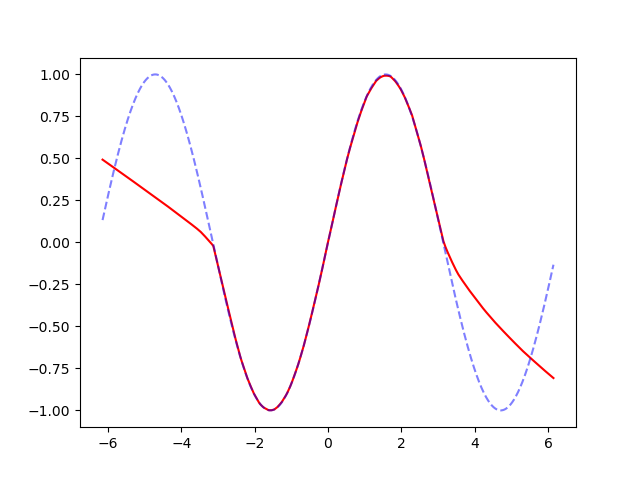
\includegraphics[width=0.5\textwidth]{pictures/1.png}

\end{center}

برای خطای MSE در هنگام یادگیری و بر اساس تقسیم بندی داده‌ها به قسمت‌های تست و آموزشی توسط توابع KFold در نهایت به طور میانگین در پنج Fold عدد زیر به دست آمده است:
$0.00062$

\hrulefill

تابع
 $sin(x) \times cos(x) + 1$
  که در بازه $-3.14$ تا $3.14$ یاد گرفته شده و در بازه $-6.30$ تا $6.30$ رسم شده.


\begin{center}

 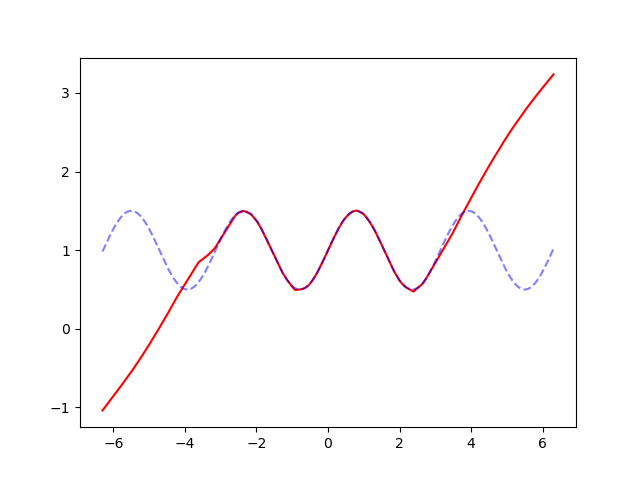
\includegraphics[width=0.5\textwidth]{pictures/2.png}

\end{center}

برای خطای MSE در هنگام یادگیری و بر اساس تقسیم بندی داده‌ها به قسمت‌های تست و آموزشی توسط توابع KFold در نهایت به طور میانگین در پنج Fold عدد زیر به دست آمده است:
$0.00106$

\newpage

\hrulefill

تابع
 $x^3 + x^2 + 3x + 1$
  که در بازه $-5$ تا $5$ یاد گرفته شده و در بازه $-10$ تا $10$ رسم شده.


\begin{center}

 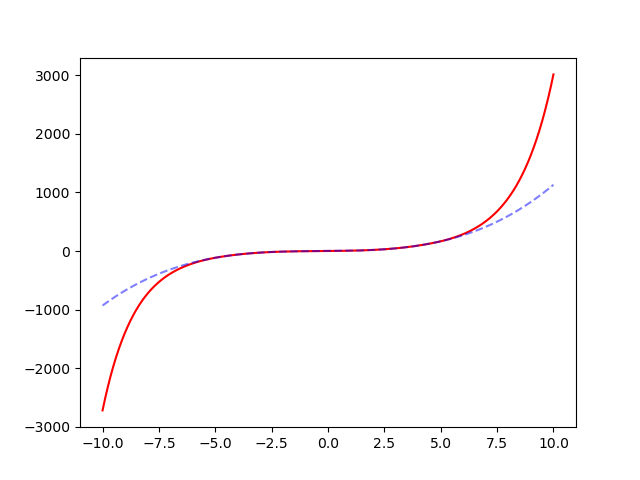
\includegraphics[width=0.5\textwidth]{pictures/3.png}

\end{center}

برای خطای MSE در هنگام یادگیری و بر اساس تقسیم بندی داده‌ها به قسمت‌های تست و آموزشی توسط توابع KFold در نهایت به طور میانگین در پنج Fold عدد زیر به دست آمده است:
$0.0086$




\hrulefill

تابع
 $\sin^{2} (x) + \cos(x) + \ln(x)$
  که در بازه $0.1$ تا $6.28$ یاد گرفته شده و در بازه $0.1$ تا $12.5$ رسم شده.


\begin{center}

 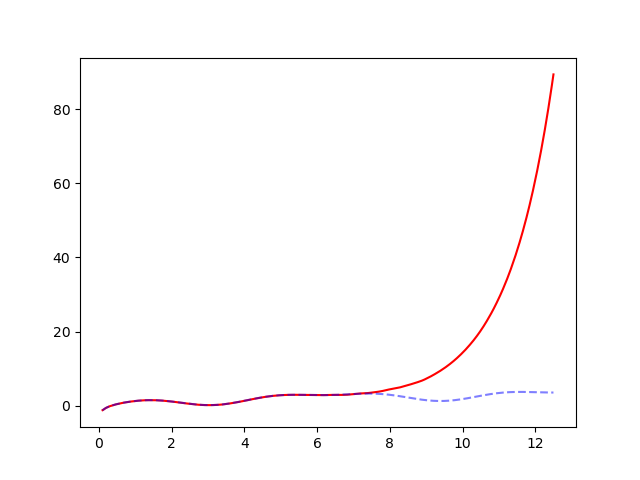
\includegraphics[width=0.5\textwidth]{pictures/4.png}

\end{center}

برای خطای MSE در هنگام یادگیری و بر اساس تقسیم بندی داده‌ها به قسمت‌های تست و آموزشی توسط توابع KFold در نهایت به طور میانگین در پنج Fold عدد زیر به دست آمده است:
$ 0.0017$



\hrulefill


تابع
 $x \times \ln(x)$
  که در بازه $0.1$ تا $10$ یاد گرفته شده و در بازه $0.1$ تا $20$ رسم شده.


\begin{center}

 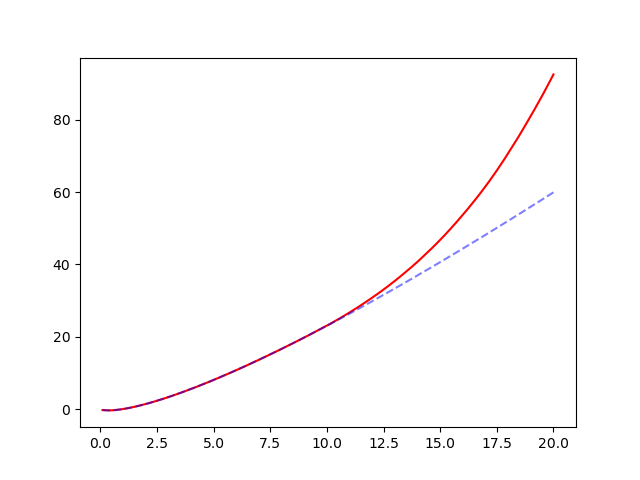
\includegraphics[width=0.5\textwidth]{pictures/5.png}

\end{center}

برای خطای MSE در هنگام یادگیری و بر اساس تقسیم بندی داده‌ها به قسمت‌های تست و آموزشی توسط توابع KFold در نهایت به طور میانگین در پنج Fold عدد زیر به دست آمده است:
$ 0.000637$


\hrulefill

از نظر زمانی، اجرای تمامی موارد با $Epoch = 6$ و با \lr{Cross Validation} به صورت $5-Fold$ با $20$ هزار داده حدود $30$ ثانیه و با $1000$ داده  حدود $2$ ثانیه زمان می‌برد. طبیعتاً دقت حالت $20$ هزار داده بیش‌تر است ولی دقت حالتی که با $1000$ داده عملیات Learning را انجام داده هم بسیار خوب و قابل قبول است

نکته مهمی که از این نتایج می‌توان به دست آورد، این است که با یادگیری از طریق این روش، می‌توان به دقت خوبی در پیش بینی رفتار تابع درون بازه‌ای که عملیات یادگیری در آن انجام شده است رسید. به عبارت دیگر با کمک این روش، می‌توان عملیات درون یابی را به شکل بسیار خوبی به انجام رساند. 

با این حال برای خارج از بازه تعیین شده، عملکرد چندان قابل قبول نیست. البته این موضوع خیلی هم دور از انتظار نیست. عملاً اگر ما هیچ اطلاعی از فرم تابع‌های ورودی نداشته باشیم و صرفاً بخواهیم با یک سیستم کلی هر تابعی که داده می‌شود را مدل کنیم، نمی‌توان انتظار داشت که برون یابی به شکل خوبی انجام بشود. بی‌شمار تابع می‌توان مثال زد که مثلا رفتار آن‌ها در بازه $-\pi$ تا $pi$ مشابه $sin(x)$ باشد اما خارج از این رفتاری کاملاً متفاوت داشته باشند و مثلا رفتار نمایی پیدا کنند. از این رو از شبکه عصبی که در بازه $[a,b]$ یادگیری را انجام داده است، نمی‌توان انتظار داشت که بتواند در خارج بازه درون یابی انجام بشود. مخصوصاً این که شبکه عصبی به صورت \lr{General Purpose} تهیه شده که هر تابعی را بتواند درون یابی کند و هیچ اطلاعی از فرم توابعی که به آن ورودی داده می‌شود، وجود ندارد. 

در کل می‌توان گفت که برای شبکه عصبی که در بالا نوشته‌ایم، می‌توان به خوبی روی قابلیت‌های درون یابی آن حساب باز کرد ولی برای برون یابی نمی‌توان به شکل عمومی از آن بهره برد. البته باید توجه کرد که عملاً هیچ روش ریاضی که به طور دقیق بتواند حاصل برون یابی را به شکل عمومی تضمین کند وجود ندارد و برای هر روشی، می‌توان به راحتی مثال نقض‌هایی آورد که روش استفاده شده روی آن جوابگو نباشند. از این رو نمی‌توان قدرت و توانایی کلی شبکه عصبی را به خاطر این موضوع زیر سؤال برد.



\newpage

\section{بخش دوم}

\subsection{توضیحات کد}
بخش عمده‌این بخش مانند قسمت قبل است. صرفاً به کانستراکتور کلاس، یک مورد جدید به نام \lr{noise\_mult} اضافه شده است که بیانگر ضریب نویز است. مثلا اگر این ضریب $0.2$ باشد، در اثر نویز عدد $100$ می‌تواند تبدیل به عددی بین $80$ تا $120$ بشود. یعنی عدد $x$ در اثر ضریب نویز $n$ به عددی بین $x(1-n)$ تا $x(1+n)$ نگاشت خواهد شد.

تابع تولید کننده نویز به این صورت است:


\begin{latin}
\begin{python}[language=Python]

   def noise_adder(self, number):
        noise_multiplier = (random.random() - 0.5) * 2 * self.noise_mult
        return number * (1 + noise_multiplier)
\end{python}

\end{latin}

که عددی تصادفی بین $-1$ تا $1$ را در \lr{noise\_mult} ضرب می‌کند و سپس با فرمولی که بالا توضیح داده شد، داده اصلی که در ورودی آن آمده است را نویز دار می‌کند.

ساختار تابع تولید کننده دیتاست هم تغییر کوچکی داشته است:


\begin{latin}
\begin{python}[language=Python]

def initial_dataset_maker(self, with_noise=False):
        X = np.linspace(self.train_low, self.train_high, num=self.NUMBER_OF_SAMPLES)
        y = self.function(X)
        if with_noise:
            y = np.array(list(map(lambda x: self.noise_adder(x), y)))
        p = np.random.permutation((self.NUMBER_OF_SAMPLES))
        self.X = X[p]
        self.y = y[p]
\end{python}

\end{latin}

به طور پیش‌فرض حالت $with\_noise$ آن غیرفعال است ولی هنگام فراخوانی با حالت Noise دار از طریق GUI این مقدار true خواهد بود و به تک‌تک داده‌های تولید شده به عنوان $y$ نویز اضافه خواهد شد.

بقیه روند این قسمت مانند بخش قبل است.


\newpage
\subsection{نتایج}

در ادامه نتایج حاصل از اجرا را به ازای noise های مختلف برای تابع $sin(x) \times cos(x) + 1$ آورده‌ام. بازه یادگیری $-3.14$ تا $3.14$ و بازه رسم نمودار $-6.3$ تا $6.3$ بوده است. (نمودار آبی تابع اصلی و قرمز تابع پیش بینی شده توسط شبکه عصبی‌ای است که یادگیری آن با داده‌های نویزدار صورت گرفته)


با ضریب نویز $0.1$: 
\begin{center}

 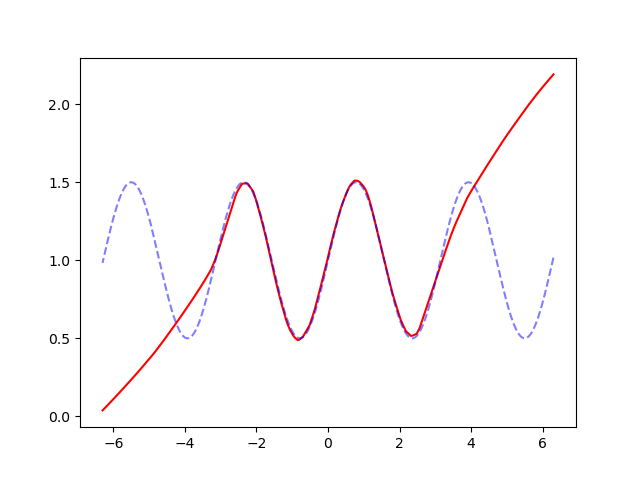
\includegraphics[width=0.5\textwidth]{pictures/6.png}

\end{center}

برای خطای MSE در هنگام یادگیری و بر اساس تقسیم بندی داده‌ها به قسمت‌های تست و آموزشی توسط توابع KFold در نهایت به طور میانگین در پنج Fold عدد زیر به دست آمده است:
$ 0.005$



\hrulefill


با ضریب نویز $0.5$: 
\begin{center}

 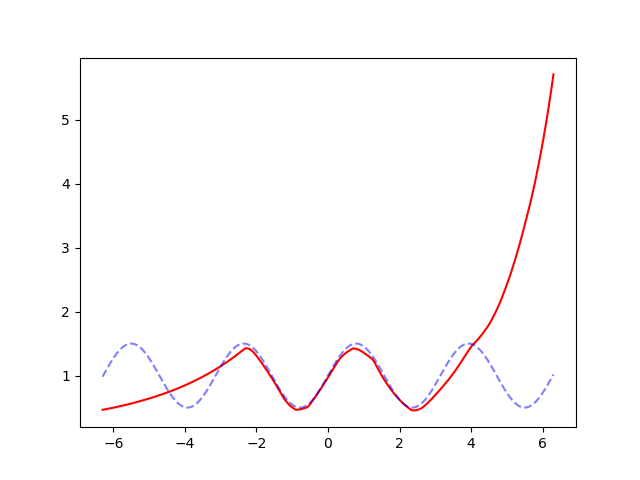
\includegraphics[width=0.5\textwidth]{pictures/7.png}

\end{center}

برای خطای MSE در هنگام یادگیری و بر اساس تقسیم بندی داده‌ها به قسمت‌های تست و آموزشی توسط توابع KFold در نهایت به طور میانگین در پنج Fold عدد زیر به دست آمده است:
$ 0.10275$

مشاهده می‌کنیم که در این حالت اختلاف‌ها بیش‌تر شده و در نتیجه یادگیری، مقادیر برون یابی شده خیلی رشد شدیدی پیدا کرده‌اند، به شکلی که مقیاس نمودار عوض شده است.





\hrulefill

\newpage

با ضریب نویز $1.0$: 
\begin{center}

 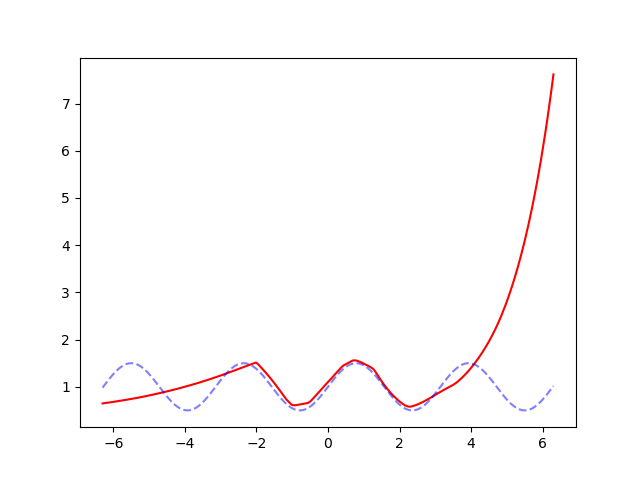
\includegraphics[width=0.5\textwidth]{pictures/8.png}

\end{center}

برای خطای MSE در هنگام یادگیری و بر اساس تقسیم بندی داده‌ها به قسمت‌های تست و آموزشی توسط توابع KFold در نهایت به طور میانگین در پنج Fold عدد زیر به دست آمده است:
$ 0.387987$



\hrulefill



با ضریب نویز $2.0$: 
\begin{center}

 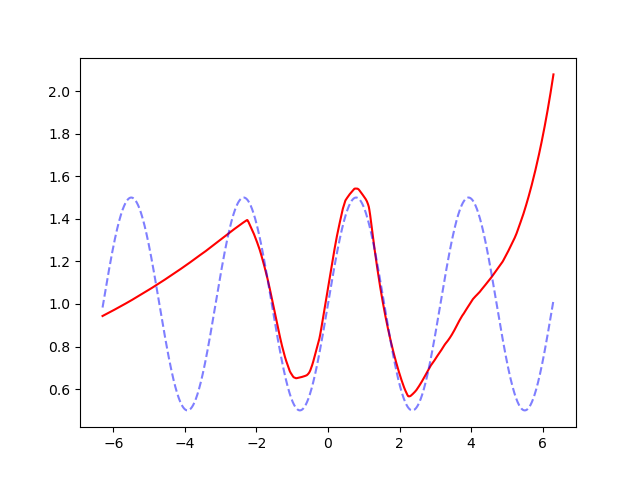
\includegraphics[width=0.5\textwidth]{pictures/9.png}

\end{center}

برای خطای MSE در هنگام یادگیری و بر اساس تقسیم بندی داده‌ها به قسمت‌های تست و آموزشی توسط توابع KFold در نهایت به طور میانگین در پنج Fold عدد زیر به دست آمده است:
$ 1.52866$

با $2$ برابر شدن سطح نویز، خطا $3$ برابر شده است.

\hrulefill


مشاهده‌ای که داریم، این است که شبکه عصبی در حالت‌هایی که میزان نویز تا حد معقولی خوب بوده و خیلی زیاد نبوده، همچنان توانسته به شکل خوبی تابع را در بازه اصلی که داده شده یاد بگیرد. اما در حالت‌هایی که نویز خیلی زیاد شده، عملکرد نهایی جالب نیست. هر چند نمی‌توان انتظار داشت وقتی دو برابر مقدار داده‌ها بتوانیم نویز داشته باشیم، شبکه عصبی بتواند خیلی خوب چنین داده‌های نویزداری را یاد بگیرد. به هر حال می‌توان از شبکه عصبی برای داده‌های نویز داری که سطح نویز آن‌ها نسبتاً معقول باشد استفاده کرد و نتیجه خوبی به دست آورد.

\section{بخش سوم}
\subsection{توضیحات کد}

کد این بخش تغیری خاصی نسبت به بخش اول ندارد. صرفاً این بار برای مواردی نظیر \lr{train\_low} و موارد مشابه، بازه به عنوان ورودی داده می‌شود و به کانستراکتور هم متغیری به نام \lr{NUMBER\_OF\_FEAUTRES} اضافه شده که تعداد متغیرها را مشخص می‌کند. تنها تغییر اصلی در بخش رسم تابع بوده که برای رسم سه بعدی آن، کد به این شکل در آمده است.


\begin{latin}
\begin{python}[language=Python]

    def plot(self):
        myRange = np.random.uniform(self.plot_low, self.plot_high,
                                    (self.NUMBER_OF_SAMPLE_FOR_PLOT,
                                     self.NUMBER_OF_FEAUTRES))
        actualZ = self.function(*myRange)
        myZ = self.model.predict(myRange)
        actualZ = actualZ.reshape(self.NUMBER_OF_SAMPLE_FOR_PLOT)
        myZ= myZ.reshape(self.NUMBER_OF_SAMPLE_FOR_PLOT)

        fig = plt.figure()
        ax = fig.gca(projection='3d')
        ax.plot_trisurf(myRange[:, 0], myRange[:, 1], myZ, alpha=0.6)
        ax.plot_trisurf(myRange[:, 0], myRange[:, 1],
         actualZ, alpha=0.5)
        return fig
\end{python}

\end{latin}

نکته مورد توجه این است که به دلیل تعداد زیاد داده‌های رسم، ممکن است رسم نمودار اندکی زمان ببرد. شاید به نظر برسد که نرم افزار قفل کرده است ولی این طور نیست.


\newpage

\subsection{نتایج}

در نمودارها، بخش آبی رنگ حاصل شبکه عصبی و بخش قرمز رنگ حاصل اعمال تابع واقعی است.



برای تابع $sin(x) + sin(y)$ در بازه آموزش $-3.14$ تا $3.14$ برای هر دو متغیر و بازه رسم $-6.3$ و $6.3$ برای هر دو


\begin{center}

 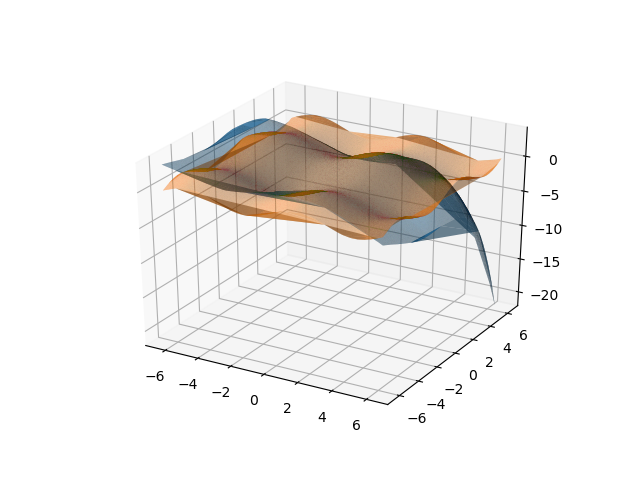
\includegraphics[width=0.5\textwidth]{pictures/10.png}

\end{center}

برای خطای MSE در هنگام یادگیری و بر اساس تقسیم بندی داده‌ها به قسمت‌های تست و آموزشی توسط توابع KFold در نهایت به طور میانگین در پنج Fold عدد زیر به دست آمده است:
$ 0.00065$


\hrulefill



برای تابع $sin(x) + sin(y)$ در بازه آموزش $-3.14$ تا $3.14$ برای هر دو متغیر و بازه رسم $-6.3$ و $6.3$ برای هر دو


\begin{center}

 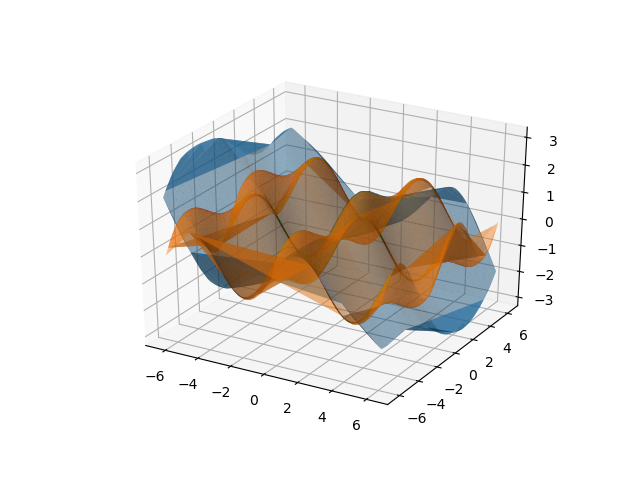
\includegraphics[width=0.5\textwidth]{pictures/11.png}

\end{center}

برای خطای MSE در هنگام یادگیری و بر اساس تقسیم بندی داده‌ها به قسمت‌های تست و آموزشی توسط توابع KFold در نهایت به طور میانگین در پنج Fold عدد زیر به دست آمده است:
$ 0.00212$


\hrulefill


\newpage

برای تابع $x+y$ در بازه آموزش $-5$ تا $5$ برای هر دو متغیر و بازه رسم $-10$ و $10$ برای هر دو


\begin{center}

 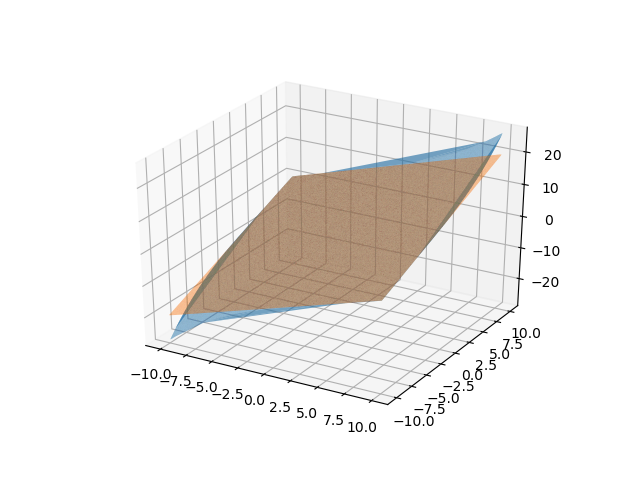
\includegraphics[width=0.5\textwidth]{pictures/12.png}

\end{center}

برای خطای MSE در هنگام یادگیری و بر اساس تقسیم بندی داده‌ها به قسمت‌های تست و آموزشی توسط توابع KFold در نهایت به طور میانگین در پنج Fold عدد زیر به دست آمده است:
$  0.00057$



\hrulefill

برای تابع $sin(x) + sin(y) + sin(z)$ در بازه آموزش $-3.14$ تا $3.14$ برای هر سه متغیر و بازه رسم $-6.3$ و $6.3$ برای هر سه اما رسم به صورت دو بعدی بر اساس $x$ و $y$ انجام شده است. متغیر سوم ثابت نبوده است ولی امکان نمایش آن هم وجود ندارد. به دلیل همین ثابت نبودن متغیر سوم، شکل تولید شده خیلی جالب نیست. هر چند همچنان می‌توان تطابق بسیار خوب را حداقل در ناحیه‌ای که یادگیری در آن صورت گرفته شاهد بود. از این رو برای نمایش بهتر دو عکس قرار گرفته که در دیگر، بازه رسم نمودار را هم محدود به $-3.14$ تا $3.14$ کرده‌ام که نتیجه بهتری قابل نمایش باشد. زیرا در خارج آن، برون یابی به خوبی صورت نمی‌گیرد. (و البته همان طور که گفتم، از یک شبکه عصبی که کاملاً \lr{General Purpose} باشد و اطلاعی از فرم توابع نداشته باشد، نمی‌توان انتظار برون یابی خیلی عجیب و غریبی را داشت. در بازه‌ای که محدود شده است، شاهد تطابق خوبی هستیم.


\begin{center}

 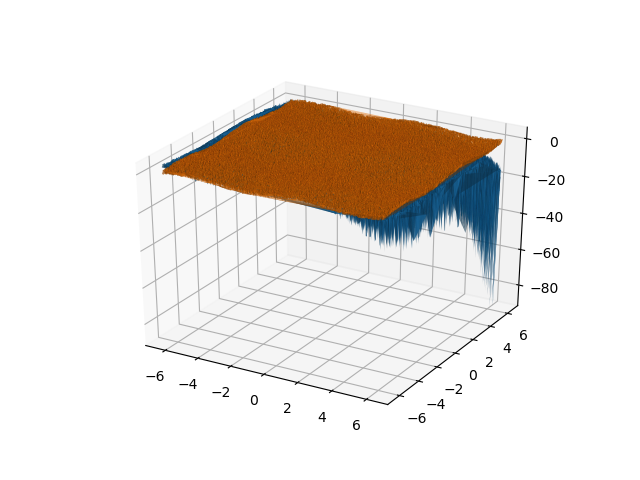
\includegraphics[width=0.5\textwidth]{pictures/13.png}

\end{center}

\begin{center}

 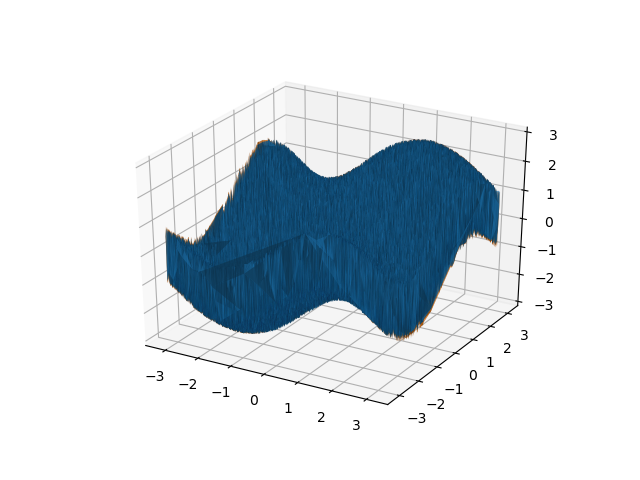
\includegraphics[width=0.5\textwidth]{pictures/14.png}

\end{center}

برای خطای MSE در هنگام یادگیری و بر اساس تقسیم بندی داده‌ها به قسمت‌های تست و آموزشی توسط توابع KFold در نهایت به طور میانگین در پنج Fold عدد زیر به دست آمده است:
$ 0.021430$


\hrulefill

در نهایت در حالت چند متغیره هم شاهد این هستیم که از بعد درون یابی، شبکه عصبی به خوبی عمل می‌کند و عملکردی نسبتاً خوبی مانند بخش‌های قبل دارد.


\newpage

\section{بخش چهارم}
\subsection{توضیحات کد}
کدهای این بخش با تغییراتی همراه بوده‌اند. اول این که یکسری موارد نظیر \lr{train\_low} و موارد مشابه از کانستراکتور حذف شده و در عوض address اضافه شده است که آدرس فایل را مشخص می‌کند. فایلی که من استفاده کردم، با استفاده از Paint رسم شده است و از روی کاغذ نیست. دلیل اصلی این امر این بوده که به جای به دست آوردن دستی نقاط بتوان توابعی نوشت که مقادیر مختصات را به دست بیاورد. توابع مورد استفاده بدین شرح هستند:



\begin{latin}
\begin{python}[language=Python]


    def initial_dataset_maker(self):
        img = Image.open(self.address, 'r')
        img = np.array(img.convert('L'))
        height, width = img.shape

        self.width = width
        self.height = height

        r = np.random.randint(0, width, width // 4)
        r = np.sort(r)

        y_s = np.array(list(map(lambda x:
         self.vertical_scanner(img, x, height), r)))

        first, last = self.find_first_last_valid(y_s, height)
        y_s = y_s[first:last]
        r = r[first:last]

        y_s = (height - y_s)

        new_len = len(y_s)
        p = np.random.permutation((new_len))
        self.X = r[p] / width
        self.y = y_s[p] / height
\end{python}

\end{latin}

این تابع عکس را لود کرده و به کمک توابع نوشته شده دیگر نظیر \lr{vertical\_scanner} و \lr{find\_first\_last\_valid} مقادیر بالایی‌ترین خط را می‌خواند و در نهایت آن‌ها را بر اساس طول و عرض عکس اسکیل و نرمالایز کرده و هم $x$ و هم $y$ را به بازه صفر تا یک می‌برد. نمونه برداری از $\frac{1}{4}$
نقاط عکس صورت می‌گیرد.


جزییات توابع کمکی مورد استفاده به این شرح است:


\begin{latin}
\begin{python}[language=Python]



   def vertical_scanner(self, img: np.array, col, height):
        for i in range(height):
            if (img[i, col] == 0):
                return i
        return height

    def find_first_valid(self, arr: np.array, invalid_number):
        size = len(arr)
        for i in range(size):
            if (arr[i] != invalid_number):
                return i

    def find_last_valid(self, arr: np.array, invalid_number):
        size = len(arr) - 1
        for i in range(size, -1, -1):
            if (arr[i] != invalid_number):
                return i

    def find_first_last_valid(self, arr, invalid_number):
        return self.find_first_valid(arr, invalid_number),
         self.find_last_valid(arr, invalid_number)

\end{python}

\end{latin}

همچنین تابع رسم هم اندکی عوض شده است و با کمک تابع \lr{all\_points} تابع \lr{plot} کار خود را انجام می‌دهد:


\begin{latin}
\begin{python}[language=Python]


 def all_points(self):
        img = Image.open(self.address, 'r')
        img = np.array(img.convert('L'))
        height, width = img.shape

        r = list(range(0, width))
        r = np.sort(r)

        y_s = np.array(list(map(lambda x:
         self.vertical_scanner(img, x, height), r)))

        first, last = self.find_first_last_valid(y_s, height)
        y_s = y_s[first:last]
        r = r[first:last]

        r = r
        y_s = (height - y_s)

        return r / width, y_s / height

    def plot(self):
        fig = plt.figure()
        myRange = np.linspace(0, 1, self.width // 2)
        myY = self.model.predict(myRange)
        plt.plot(myRange, myY, '-r')
        actualx, actualY = self.all_points()
        plt.plot(actualx, actualY, '--b', alpha=0.5)
        return fig

\end{python}

\end{latin}


در نهایت ساختار مدل شبکه عصبی هم تغییراتی داشته است:

\begin{latin}
\begin{python}[language=Python]


 model = keras.Sequential()
            model.add(keras.layers.Dense(1, input_dim=1,
             activation='linear', kernel_initializer='he_uniform'))
            model.add(keras.layers.Dense(40, activation='relu',
             kernel_initializer='he_uniform'))
            model.add(keras.layers.Dense(40, activation='relu',
             kernel_initializer='he_uniform'))
            model.add(keras.layers.Dense(40, activation='relu',
             kernel_initializer='he_uniform'))
            model.add(keras.layers.Dense(1 , activation = "linear"))

            opt = keras.optimizers.Nadam(learning_rate=0.01)

            model.compile(optimizer=opt, loss='mse')

\end{python}

\end{latin}

تعداد لایه‌ها و Node های آنان کمتر شده است. همچنین \lr{Kernel Initializer} به صورت تابع یونیفرم در آمده و به جای توزیع نرمال از توزیع یکنواخت عدد تصادفی تولید می‌شود. برای اپتیمایزر هم به جای Adam از Nadam استفاده شده که تفاوت کمی با Adam دارد و نرخ یادگیری آن هم به جای $0.001$ روی $0.01$ تنظیم شده است.

همچنین تعداد Epoch هایی که برای اجرای پیش فرض در نظر گرفته شده است و توصیه می‌شود هم به جای قبلی‌ها که $5$ یا $6$ بود در این حالت $50$ است. هر چند به دلیل ساختار شبکه از نظر زمانی سرعت کلی اجرا بالا است.





\newpage

\subsection{نتایج}

در نمودارها، بخش آبی رنگ حاصل شبکه عصبی و بخش قرمز رنگ حاصل اعمال تابع واقعی است.


شکل اولیه این بوده است:



\begin{center}

 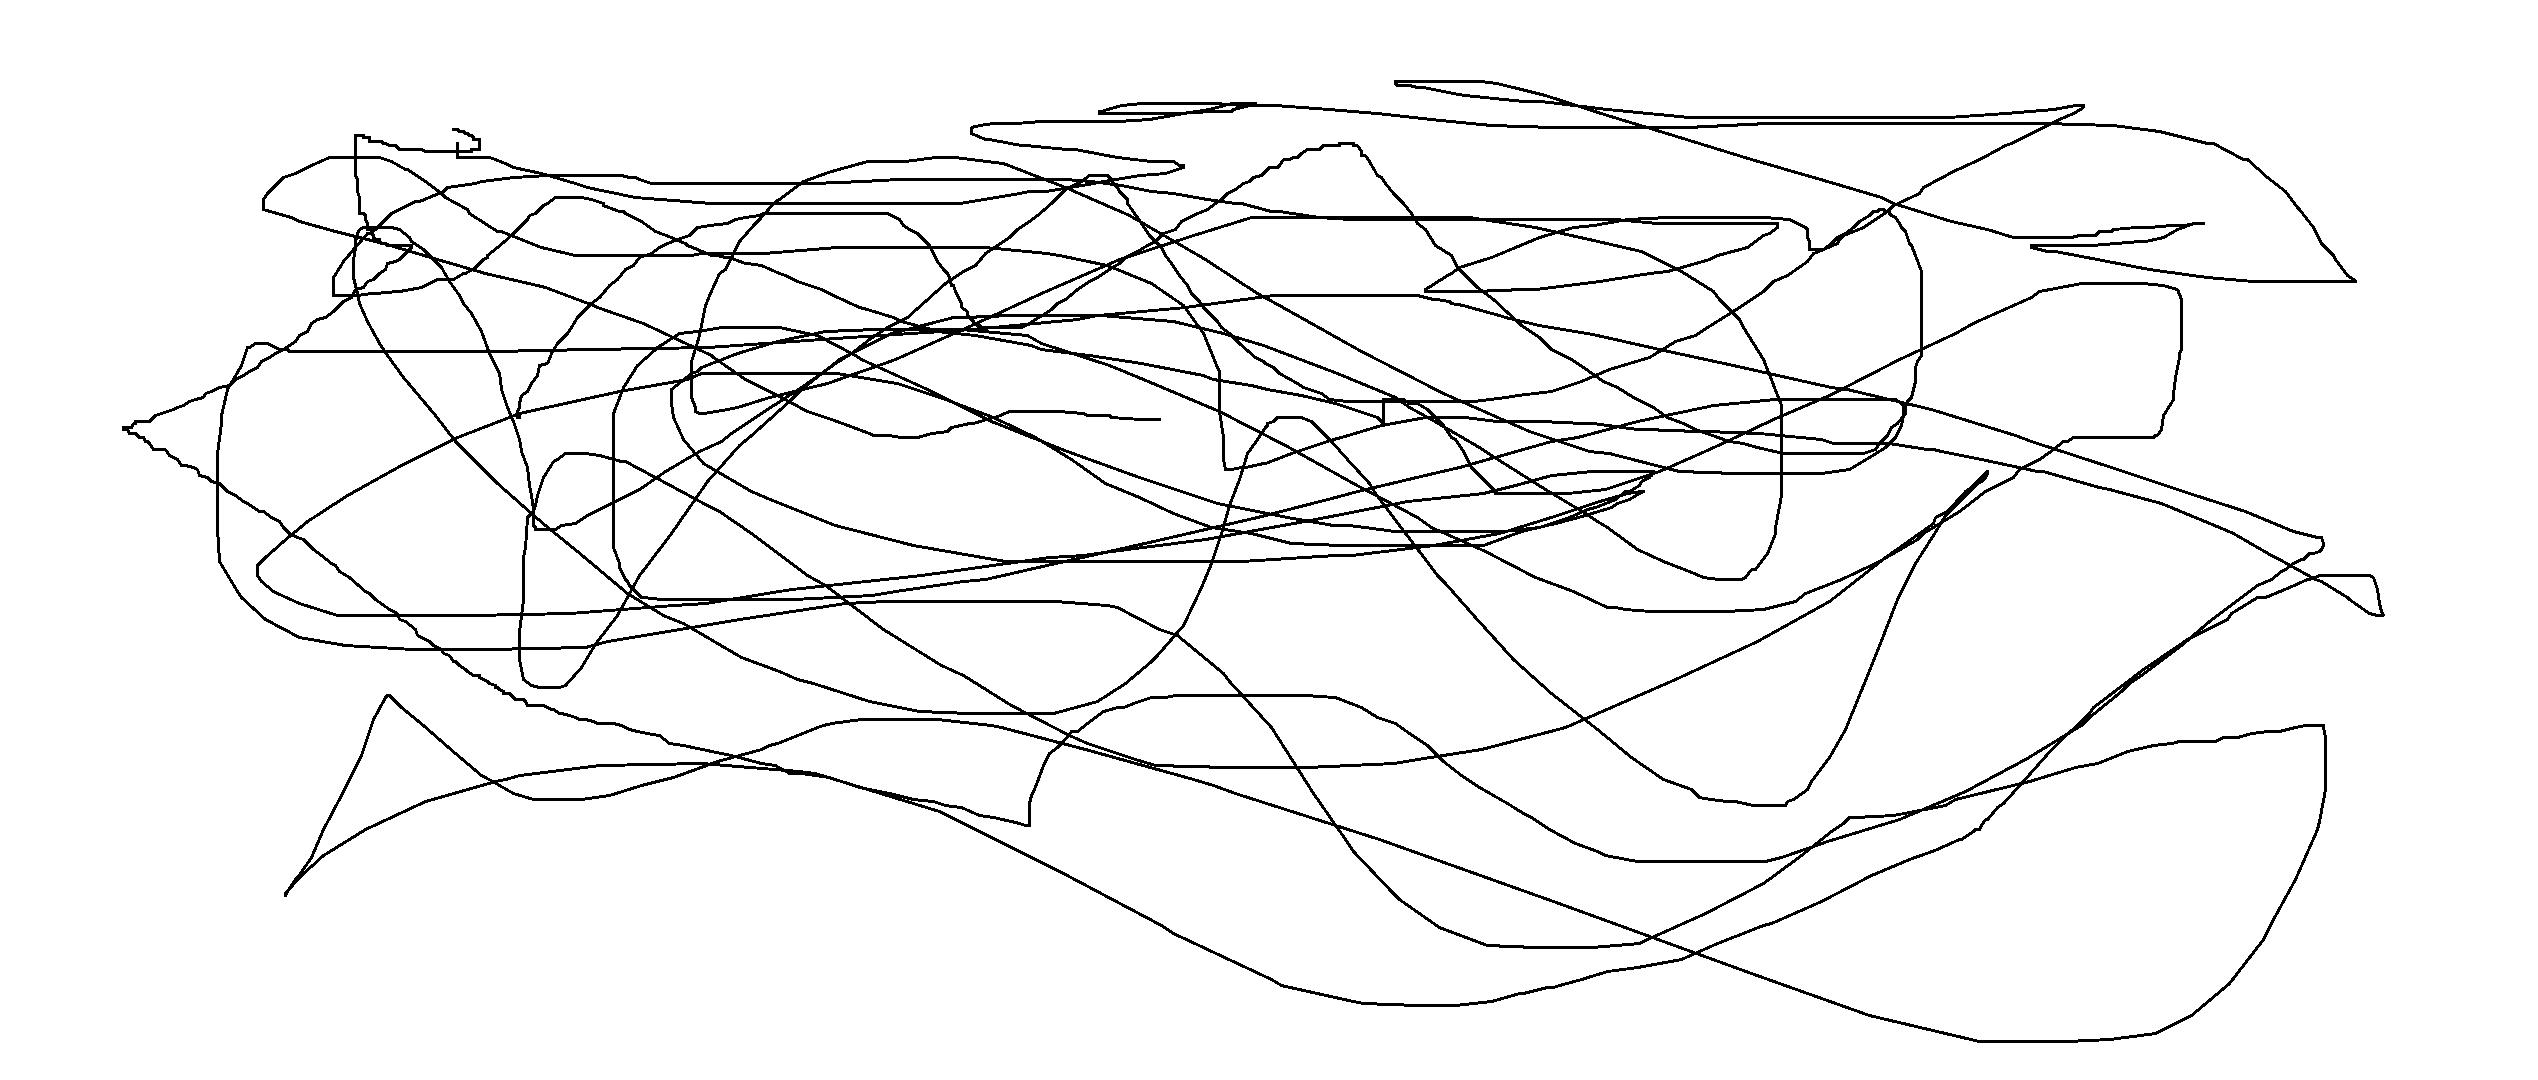
\includegraphics[width=0.5\textwidth]{pictures/16.png}

\end{center}

بعد از نرمالایز شدن به بازه $0$ و $1$ و یادگیری حاصل به این صورت در آمده است. 


\begin{center}

 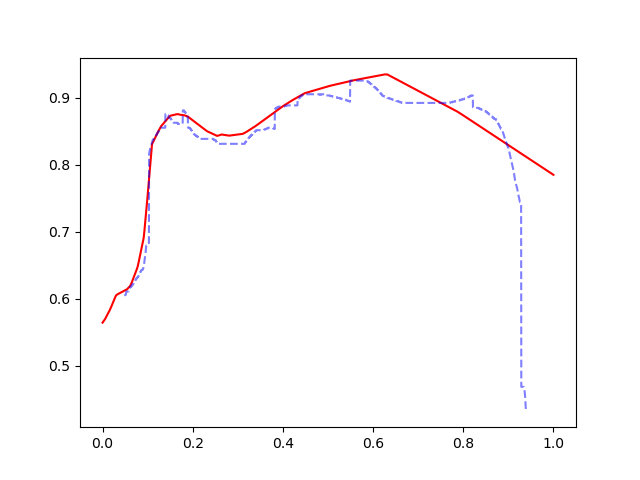
\includegraphics[width=0.5\textwidth]{pictures/15.png}

\end{center}


برای خطای MSE در هنگام یادگیری و بر اساس تقسیم بندی داده‌ها به قسمت‌های تست و آموزشی توسط توابع KFold در نهایت به طور میانگین در پنج Fold عدد زیر به دست آمده است:
$ 0.00427$




\hrulefill


در این جا مشاهده می‌کنیم که کلیت شکل به درستی تشخیص داده شده. با این وجود، چیزی که باعث ایجاد مشکل عمده شده است، همان پرش‌های ناگهانی است که در مستند طراحی پروژه هم به آن اشاره شده بود. وجود این پرش‌های ناگهانی در تصویر، باعث شده که شبکه عصبی در آن قسمت‌ها نتواند خوب عمل کند و مخصوصاً در تکه آخر که شاهد یک پرش خیلی بزرگ هستیم، در بازه کوچکی اصلاً عملکرد شبکه خوب نیست.

در ادامه نمونه حاصل از یک تصویر نسبتاً پیوسته شبه سینوسی هم آورده شده که میانگین خطای 
 $0.0006$
 برای آن به دست آمد و نتیجه نهایی نیز بهتر از تصویر قبلی است که نشان می‌دهد اصلی‌ترین مشکل شکل قبلی، پرش‌های ناگهانی موجود در آن است که باعث به مشکل خوردن شبکه عصبی شده است.
 
 
 \begin{center}

 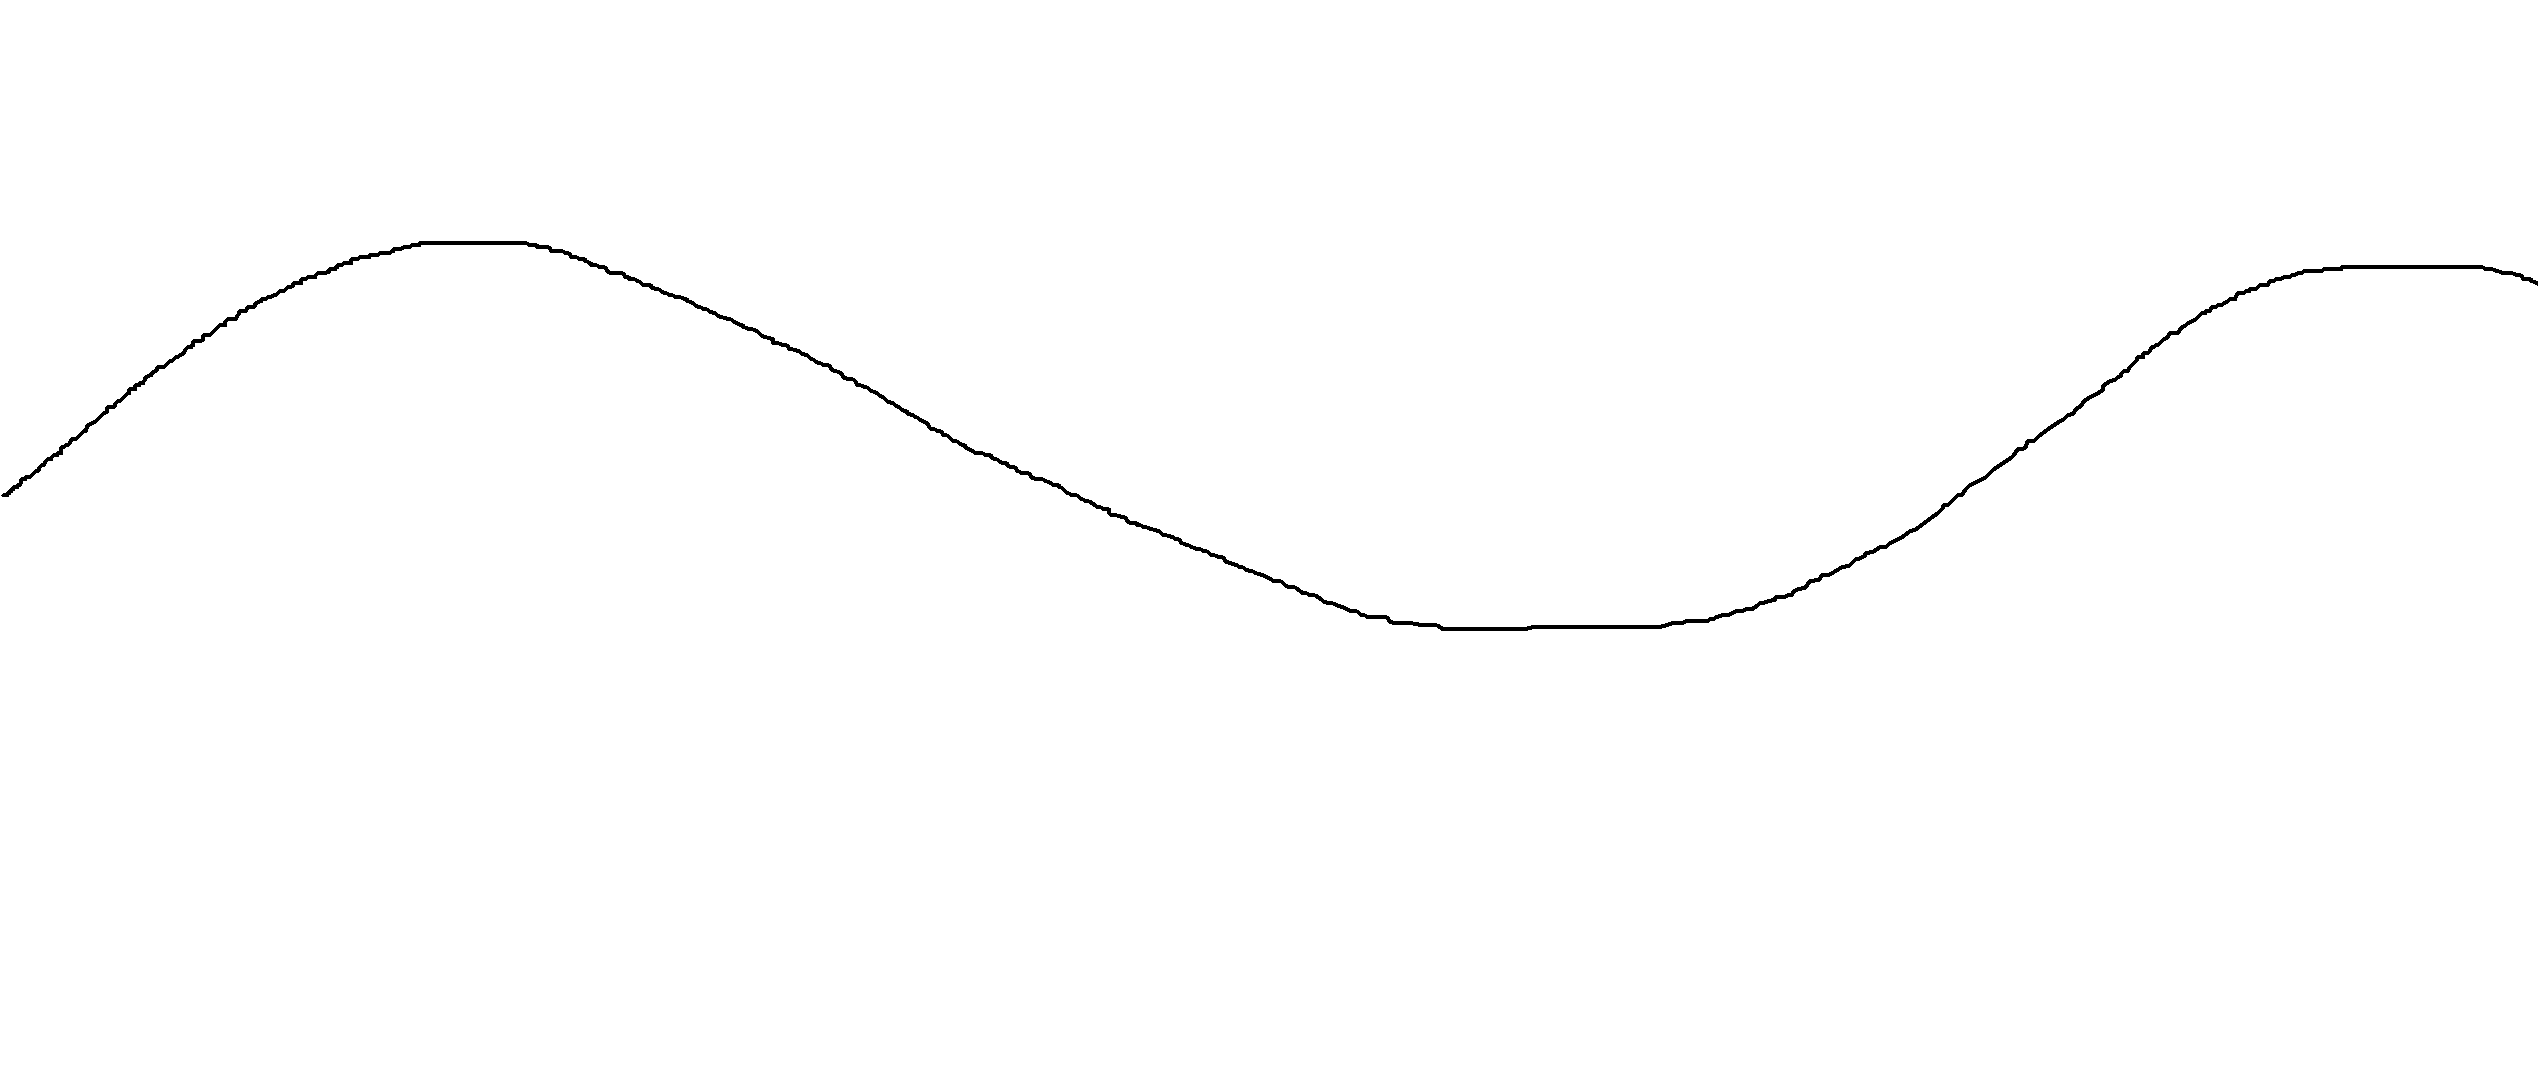
\includegraphics[width=0.5\textwidth]{pictures/17.png}

\end{center}

بعد از نرمالایز شدن به بازه $0$ و $1$ و یادگیری حاصل به این صورت در آمده است. 


\begin{center}

 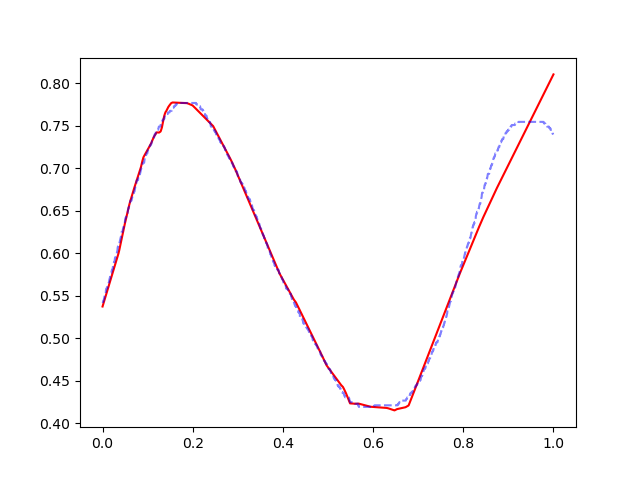
\includegraphics[width=0.5\textwidth]{pictures/18.png}

\end{center}
\newpage


\section{بخش پنجم}

\subsection{توضیحات کد}

عمده تغییرات این بخش مربوط به نحوه لود کردن دیتاست و همچنین ساختار شبکه عصبی است.

دیتاست مورد استفاده MNIST بوده است که شامل $60000$ رقم دست نویس انگلیسی است. این دیتاست درون خود Keras قرار دارد و برای لود آن از این تابع استفاده شده است:

\begin{latin}
\begin{python}[language=Python]

  def load_mnist(self):
        MNIST_DS = keras.datasets.mnist
        (train_images, train_labels), (test_images, test_labels)
         = MNIST_DS.load_data()

        train_images = train_images / 255
        test_images = test_images / 255

        images = np.concatenate((train_images, test_images), axis=0)
        labels = np.concatenate((train_labels, test_labels), axis=0)

        self.images = images
        self.labels = labels

\end{python}

\end{latin}

در ساختار شبکه هم تغییراتی داشته‌ایم:


\begin{latin}
\begin{python}[language=Python]

 model = keras.Sequential()
            model.add(keras.layers.Flatten(input_shape=(28, 28)))
            model.add(keras.layers.Dense(28*28+2,
             activation='sigmoid'))
            model.add(keras.layers.Dense(10, activation='softmax'))

            model.compile(loss=self.LOSS_FUNCTION, metrics=['accuracy'],
             optimizer='adam')

\end{python}

\end{latin}


تابعی که برای محاسبه خطا استفاده شده، تابعی به نام \lr{sparse\_categorical\_loss} است که تابع پیشنهادی خود Keras برای سیستم‌های دسته بندی و Classifier محسوب می‌شود. شکل دیگری از آن هم به نام \lr{categorical\_loss} وجود دارد و تفاوت آن‌ها در این است که از حالت sparse زمانی استفاده می‌شود که هر شکل تنها به یک دسته تعلق داشته باشد و از حالت دوم زمانی استفاده می‌شود که یک شکل بتواند به چند دسته متعلق باشد که طبیعتاً در این جا حالت اول اتفاق می‌افتد. ضمناً در این مورد، علاوه بر نمایش میزان خطا به صورت چاپی، دقت یعنی درصد مواردی که به درستی تشخیص داده شده‌اند هم در Log های نوشته شده، قرار می‌گیرند.

در ساختار شبکه، در مرحله اول یک لایه داریم که داده‌ها را به صورت ماتریس $28 \times 28$ دریافت کرده و به صورت خطی $784$ تایی در می آورد. سپس یک لایه سیگمویدی با ابعاد $786$ داریم. دلیل استفاده از $786$ این بوده که اندکی بزرگ‌تر از ابعاد کلی تصویر را استفاده کنیم. در ابتدا حالت‌هایی که چند لایه سیگمویدی $100$ تایی پشت سر هم داشتیم را تست کردم و هر چند آن‌ها هم خوب بودند، اما این حالت با سرعتی معقول، دقت نسبتاً بهتری را از آن‌ها بدون ایجاد Overfit زیاد در اختیارمان می‌گذارد. در نهایت هم یک لایه softmax قرار گرفته است که احتمال حضور داده ما در هر کدام از دسته‌ها را مشخص می‌کند.


یک تابع به نام \lr{image\_predict} هم داریم که با گرفتن یک اندیس، شکل آن تصویر را نمایش داده و نتیجه پیش بینی شده توسط شبکه آموزش دیده را هم مشخص می‌کند. این تابع به صورت زیر است:

\begin{latin}
\begin{python}[language=Python]
    def image_predict(self, index):
        fig = plt.figure()
        plt.imshow(self.images[index])
        image = np.array(self.images[index]).reshape(-1, 28, 28)
        answer = self.model.predict(image)
        return fig, np.argmax(answer)
\end{python}

\end{latin}


\newpage
\subsection{نتایج}
با انجام عملیات یادگیری، شبکه نوشته شده در بالا توانست به دقت $97.7285$ درصدی به طور میانگین در بین Fold های مختلف برای داده تست و دقت $98.87$ درصدی برای داده آموزشی دست پیدا کند.

با چنین دقتی بخش عمده‌ای از اندیس‌های تصادفی که من تست کردم، نتیجه‌ای درست می‌دادند. برای همین از آن جایی که اکثر مواقع نتیجه شبکه عصبی درست بود، در زیر عکس حالتی را آورده‌ام که غلط تشخیص داده شد. بعد از تست اندیس‌های زیاد، به یک تصویر برخوردم که نتیجه غلط می‌داد و آن را در پایین آورده‌ام. با این تقریباً بعد از $40$ بار تست کردن تصاویر تصادفی مختلف، به این $1$ مورد غلط رسیدم نشان دهنده دقت بسیار خوبی است که تقریبا معادل $97.5$ درصد می‌شود که معادل همان دقتی است که الگوریتم گزارش کرده بود.


به عنوان نمونه‌ای از تشخیص اشتباه، تصویر زیر عدد $2$ بود که به اشتباه به عنوان $0$ دسته بندی شده بود.

\begin{center}

 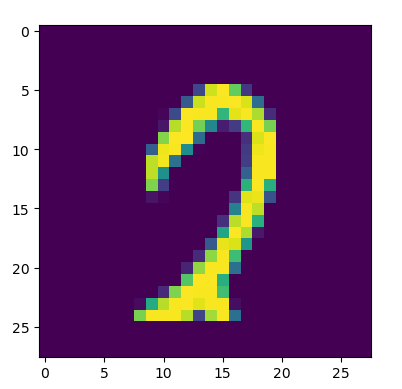
\includegraphics[width=0.5\textwidth]{pictures/19.png}

\end{center}

دلیل تشخیص اشتباه می‌تواند این باشد که در اکثر تصاویر، خط پایین دو طول بیش‌تری داشت. در این تصویر خط پایین طول کوتاهی دارد و از طرفی انحنای بالای آن شبیه بسیاری از صفرهای دیتاست است که به صورت کج نوشته شده‌اند. در نتیجه الگوریتم با وزن‌هایی که یادگرفته، این ساختار را بیش تر مشابه $0$ تشخیص داده است.



\hrulefill

\newpage

\section{بخش ششم}

\subsection{توضیحات کد}


بخش عمده تغییر این بخش مربوط به اضافه کردن توابع نویز است. پنج سطح نویزی به نام‌های 
\lr{LOW, MEDIUM, HIGH, ULTRA, ULTRA\_HIGH} برای سؤال در نظر گرفتم. در ورودی‌های کانستراکتور این سطح نویز به عنوان ورودی گرفته می‌شود. همچنین mode و type کلی نویزهای اعمال شده را هم می‌توان مشخص کرد که به طور پیش فرض noise از نوع gaussian است ولی می‌توان مثلا نوع \lr{s\&p} یا \lr{poisson} را هم امتحان کرد. هر چند عملاً gaussian با ترکیب \lr{s\&p} در حالت ultra نویز بسیار سنگینی است که می‌تواند جوابگوی تست ما برای کارکرد شبکه باشد.

 همچنین در کانستراکتور مقداری به نام \lr{NUMBER\_OF\_IMAGES\_TO\_USE}
قرار دارد که مشخص می‌کند از چه تعداد از تصاویر MNIST به طور کلی برای فرآیند یادگیری و تست استفاده شود. چون تصاویر MNIST زیاد هستند و اگر از همه آن‌ها استفاده شود، فرآیند یادگیری از آن جایی که هم ورودی و هم خروجی شامل $784$ المان است، از نظر زمانی کمی طولانی می‌شود. مقدار پیش فرض آن $10000$ است.




تابع اضافه کننده نویز به این صورت است که اگر mode ان None باشد نویز اضافه نمی‌کند، در غیر این صورت Noise را بر اساس سطح نویز تعریف شده در هنگام ساخته شدن آبجکت از این کلاس، اعمال می‌کند. برای اعمال خود نویز هم از توابع کتابخانه skimage استفاده شده است.



\begin{latin}
\begin{python}[language=Python]
 def add_noise(self, img, mode):
        gimg = img
        if mode is not None:
            if (self.noise_degree == LOW):
                gimg = skimage.util.random_noise(img,
                 mode=mode, clip=True)
            if (self.noise_degree == MEDIUM):
                gimg = skimage.util.random_noise(img,
                 mode=mode, clip=True)
                gimg = skimage.util.random_noise(gimg,
                 mode=mode, clip=True)
                gimg = skimage.util.random_noise(gimg,
                 mode=mode, clip=True)
            if (self.noise_degree == HIGH):
                gimg = skimage.util.random_noise(img, 
                mode=mode, clip=True)
                gimg = skimage.util.random_noise(gimg,
                 mode=mode, clip=True)
                gimg = skimage.util.random_noise(gimg, 
                mode=mode, clip=True)
                gimg = skimage.util.random_noise(gimg, 
                mode=mode, clip=True)
                gimg = skimage.util.random_noise(gimg,
                 mode=mode, clip=False)
            if (self.noise_degree == ULTRA):
                gimg = skimage.util.random_noise(img, 
                mode=mode, clip=True)
                gimg = skimage.util.random_noise(gimg, 
                mode=mode, clip=True)
                gimg = skimage.util.random_noise(gimg,
                 mode=mode, clip=True)
                gimg = skimage.util.random_noise(gimg,
                 mode=mode, clip=True)
                gimg = skimage.util.random_noise(gimg,
                 mode=mode, clip=False)
                gimg = skimage.util.random_noise(gimg,
                 mode='s&p', clip=False)
            if (self.noise_degree == ULTRA_HIGH):
                gimg = skimage.util.random_noise(img, 
                mode=mode, clip=True)
                gimg = skimage.util.random_noise(gimg,
                 mode=mode, clip=True)
                gimg = skimage.util.random_noise(gimg, 
                mode=mode, clip=True)
                gimg = skimage.util.random_noise(gimg,
                 mode=mode, clip=True)
                gimg = skimage.util.random_noise(gimg,
                 mode=mode, clip=False)
                gimg = skimage.util.random_noise(gimg, 
                mode='s&p', clip=False)
                gimg = Image.fromarray(np.uint8
                (cm.gist_gray(gimg) * 255))
                gimg = gimg.filter(ImageFilter.BLUR)
                gimg = np.asarray(gimg) / 255
                gray = lambda rgb: np.dot
                (rgb[..., :3], [0.299, 0.587, 0.114])
                gimg = gray(gimg)

        return gimg
\end{python}

\end{latin}

سه حالت Noise اول چندین سطح از Noise گاوسی را دارند. حالت ULTRA تعداد این سطح ها را بیش تر کرده و یک نویز \lr{Salt and Pepper} که بعضی نقاط را به طور رندوم $0$ و بعضی را $1$ هم اضافه می کند. حالت \lr{ULTRA\_HIGH} علاوه بر نویز بخش ULTRA افکت BLUR و محو شدن را هم به تصویر اضافه می کند.
 
 
 از تابع زیر برای لود کردن تصاویر MNIST و همچنین اضافه کردن Noise استفاده شده است.
 
 \begin{latin}
\begin{python}[language=Python]
  def load_noised_digits(self):
        MNIST_DS = keras.datasets.mnist
        (train_images, train_labels), (test_images, test_labels)
         = MNIST_DS.load_data()
        train_images = train_images / 255
        test_images = test_images / 255
        images = np.concatenate((train_images, test_images), axis=0)

        p = np.random.permutation((len(images)))
        images = images[p]
        images = images[0:self.NUMBER_OF_IMAGES_TO_USE]
        noised_images = np.array(list(map(lambda x:
         self.add_noise(x, self.noise_type), images))).reshape(
            -1, 28, 28)
        self.images = images
        self.noised_images = noised_images
\end{python}

\end{latin}
 
 در نهایت ساختار شبکه هم به این صورت در آمده است:
 
 
  \begin{latin}
\begin{python}[language=Python]
  model = keras.Sequential()
            model.add(keras.layers.Dense(784, activation='relu'))
            model.add(keras.layers.Dense(784 * 2,
             activation='sigmoid'))
            model.add(keras.layers.Dense(784, activation='sigmoid'))

            model.compile(loss=self.LOSS_FUNCTION, optimizer='adam')
\end{python}

\end{latin}

و در ابتدا از یک لایه relu و سپس دولایه سیگمویدی استفاده شده است.


ساختار رسم تصاویر هم تغییر کرده تا امکان رسم و مقایسه چند حالت در یک شکل مهیا بشود که کد آن به این شرح است.


  \begin{latin}
\begin{python}[language=Python]
 def enhance_image(self, index):
        image_to_enhance = self.noised_images[index]
        enhanced_image = self.model.predict
        (np.array(image_to_enhance).reshape(-1, 28 * 28))
        original_image = self.images[index]
        return image_to_enhance.reshape(28, 28),
         enhanced_image.reshape(28, 28),
          original_image.reshape(28, 28)

    def add_to_plot(self, index, axs, r, is_one_line):
        noised, enhanced, original = self.enhance_image(index)
        if (is_one_line):
            axs[0].imshow(noised)
            axs[1].imshow(enhanced)
            axs[2].imshow(original)

        else:
            axs[r, 0].imshow(noised)
            axs[r, 1].imshow(enhanced)
            axs[r, 2].imshow(original)
        return axs

    def plot(self, indices):
        r = len(indices)
        fig = plt.figure(dpi=100)
        axs = fig.subplots(r, 3)
        is_one_line = True if r == 1 else False
        for i in range(r):
            axs = self.add_to_plot(indices[i], axs, i, 
            is_one_line=is_one_line)
        if is_one_line:
            axs[0].set_title("Noised")
            axs[1].set_title("Enhanced")
            axs[2].set_title("Original")
        else:
            axs[0, 0].set_title("Noised")
            axs[0, 1].set_title("Enhanced")
            axs[0, 2].set_title("Original")

        return fig

\end{python}

\end{latin}

که تابع اول مسئول اجرای شبکه عصبی بر روی عکس بوده و دو تابع دیگر، آن‌ها را در شکل قرار می‌دهند.







\newpage
\subsection{نتایج}

نتایج اعمال نویز \lr{LOW}:

میانگین خطا \lr{MSE}: $
0.0325$

\begin{center}

 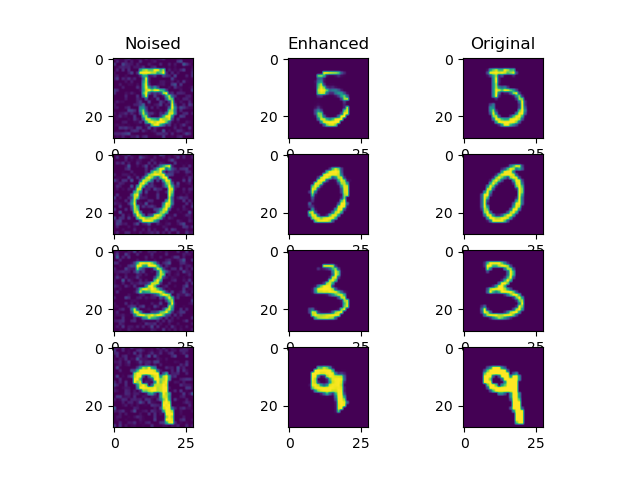
\includegraphics[width=0.5\textwidth]{pictures/20.png}

\end{center}


\hrulefill




نتایج اعمال نویز \lr{MEDIUM}:

میانگین خطا \lr{MSE}: $
0.0384$

\begin{center}

 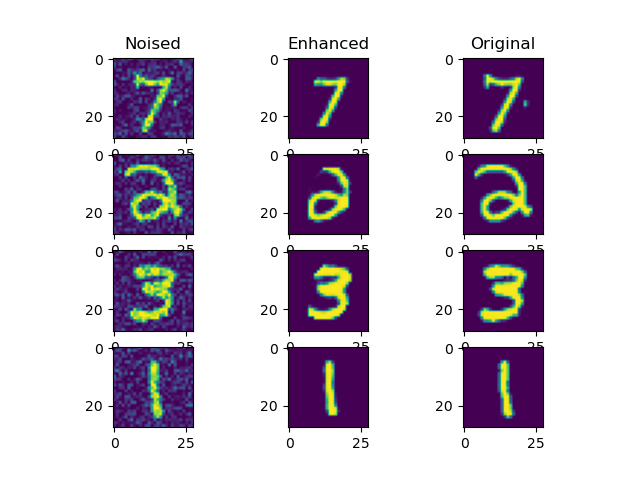
\includegraphics[width=0.5\textwidth]{pictures/22.png}

\end{center}

\hrulefill


\newpage






نتایج اعمال نویز \lr{HIGH}:

میانگین خطا \lr{MSE}: $
0.0433$

\begin{center}

 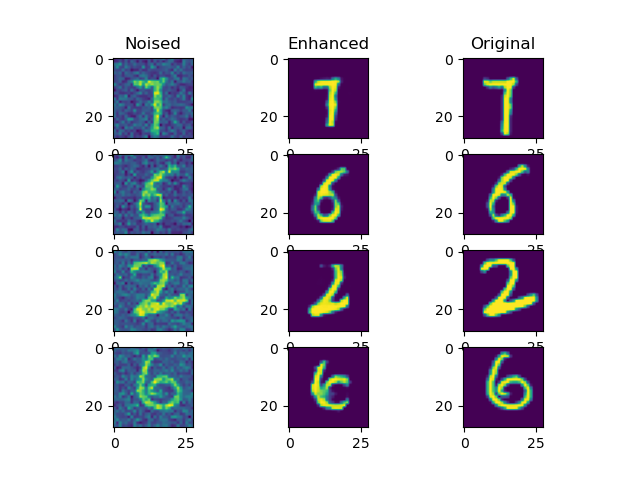
\includegraphics[width=0.5\textwidth]{pictures/23.png}

\end{center}


\hrulefill


نتایج اعمال نویز \lr{ULTRA}:

میانگین خطا \lr{MSE}: $0.051$

\begin{center}

 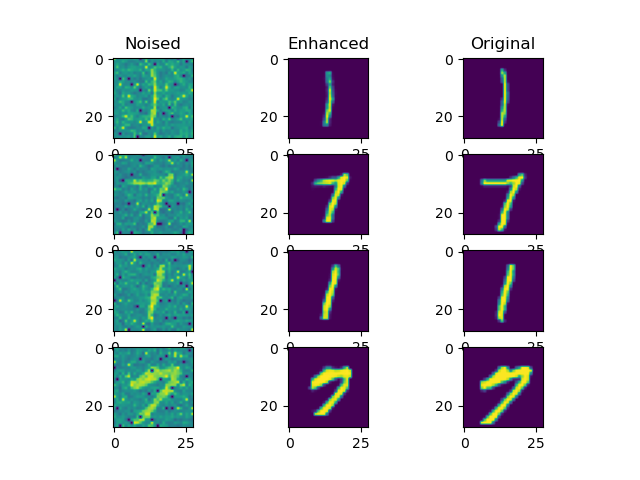
\includegraphics[width=0.5\textwidth]{pictures/21.png}

\end{center}


\hrulefill


\newpage

نتایج اعمال نویز \lr{ULTRA\_HIGH}:

میانگین خطا \lr{MSE}: $0.053$

\begin{center}

 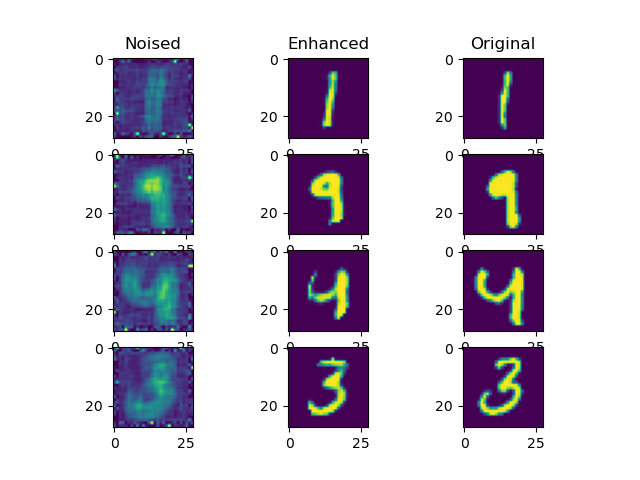
\includegraphics[width=0.5\textwidth]{pictures/30.png}

\end{center}


\hrulefill


اکثر نتایج حاصله بسیار خوب و قابل قبول هستند. سعی کرده‌ام یکی دو نمونه‌ای که خیلی عالی نبوده‌اند را هم در عکس‌ها قرار بدهم. با این وجود در کل، کیفیت بازسازی عکس‌ها از روی شکل نویزدار در اکثر مواقع بسیار خوب و عالی بوده است.

\newpage

\section{بخش هفتم}

اصلی‌ترین عنصر یک شبکه عصبی ساختار لایه‌های قرار گرفته درون آن است. در کتابخانه‌ای نظیر Keras این لایه‌ها چند ویژگی اساسی دارند، تعداد Node ها، تابع فعال ساز و همچنین \lr{Kernel Initializer}. چیزی نظیر \lr{Kernel Initializer} را معمولاً می‌توان به صورت دستی برای مسئله تعیین کرد. اما Node ها و تابع فعال ساز چیزی نیستند که بتوان برای هر مسئله‌ای به صورت دستی انتخاب کرد. مخصوصاً این که بعضی از توابع فعال ساز، نیاز به یکسری پارامتر هم دارند. هم چنین در نهایت Optimizer مورد استفاده و پارامترهای آن هم اهمیت بالایی دارند.

از طرف دیگر، در یک سیستم ژنتیک، ما مسئله را به صورت کروموزوم‌هایی مدل می‌کنیم که در اثر Crossover می‌توانند با هم ترکیب شده و بخش‌هایی از یک کروموزوم در کنار بخش‌هایی از یک کروموزوم دیگر قرار بگیرد. همچنین در عمل Mutation هم جهش‌های ناگهانی در بخش‌هایی از یک کروموزوم رخ می‌دهد. بدین ترتیب، جمعیت‌های مختلفی ایجاد شده و نسل به نسل، این فرآیندها بین جمعیت تکرار می‌شود تا به حالت مطلوب مسئله برسیم ضمناً مورد بعضی از عناصر جمعیت هم شاهد این هستیم که بدون هیچ عملی، به نسل بعد منتقل می‌شوند.


حال برای حل این مسئله، در اصل کار اصلی، مدل کردن مسئله شبکه عصبی به مسئله ژنتیک است. برای این کار، کروموزوم‌های ما در اصل همان ساختار شبکه هستند. عناصر این کروموزوم‌ها شامل این که در هر لایه چند Node و همچنین با چه توابعی قرار دارد و همچنین پارامترهای آن توابع و Optimizer نهایی مسئله می‌شود. حتی مواردی نظیر تعداد Epoch ها و \lr{Batch Size} هم می‌تواند در کروموزوم آورده شود. مانند مسئله‌ای که در پروژه ژنتیک برای به دست آوردن تابع داشتیم و شاهد توابع با چند ورودی بودیم، در این جا هم مثلا بعضی لایه‌ها با توجه به تابع فعال سازشان می‌توانند چندین پارامتر داشته باشند یا پارامتری نداشته باشند. در نهایت باید جمعیت زیادی از ساختارهای مختلف تولید شده و سیستم ژنتیک روی آن‌ها اجرا شود.

برای این که میزان شایستگی هر کروموزوم سنجیده شود، باید چند معیار مورد بررسی قرار بگیرد. اولین مورد دقت و خطای نهایی آن است. مورد بعدی، زمان اجرای آن است. مورد دیگر سطح پیچیدگی شبکه است که می‌تواند یک تابع باشد که بر اساس تعداد لایه‌ها و Node های آنان، عددی را به عنوان سطح پیچیدگی شبکه اعلام کند. طبیعتاً دقت بالاتر و زمان کمتر باعث بیش‌تر شدن شایستگی می‌شوند. همچنین بنا به مسئله، در اکثر اوقات ساختار ساده‌تر هم می‌تواند یک نشانه مثبت تلقی شود. از ترکیب این موارد، یک عدد برای شایستگی به دست می‌آید و در نهایت از این اعداد برای اجرای الگوریتم ژنتیک استفاده می‌شود.

باید توجه کرد که این روش هر چند از تست کردن دستی راحت‌تر است، اما همچنان به منابع محاسباتی زیادی نیاز دارد. با این وجود، به دلیل این که عملاً اجرای و یادگیری هر کدام از عناصر جمعیت که شبکه‌ها هستند، می‌تواند به طور مستقل صورت بگیرد، امکان موازی سازی بالایی برای عملیات‌ها وجود داشته و با استفاده از یک یا چند GPU قوی که هسته‌های CUDA فراوانی داشته باشد، می‌توان از طریق موازی سازی، با سرعت نسبتاً خوبی ساختاری تقریباً بهینه برای شبکه را یافت.

هر چند تمامی این موارد باید در عمل هم آزمایش بشود. به هر حال الگوریتم‌های ژنتیک تضمینی برای درستی جواب به ما ارائه نمی‌دهند و در نتیجه تا کل این موارد به صورت عملی و آکادمیک تست نشود، نمی‌توان با قطعیت گفت که آیا برای یک پروژه بزرگ واقعی، پیاده‌سازی الگوریتم ژنتیک برای یافتن ساختار شبکه توجیه و صرفه اقتصادی و زمانی دارد یا نه.


\section{رابط کاربری}
در این بخش توضیحاتی در مورد نحوه کار با رابط کاربری هر بخش آورده شده است.

\subsection{بخش اول}

\begin{center}

 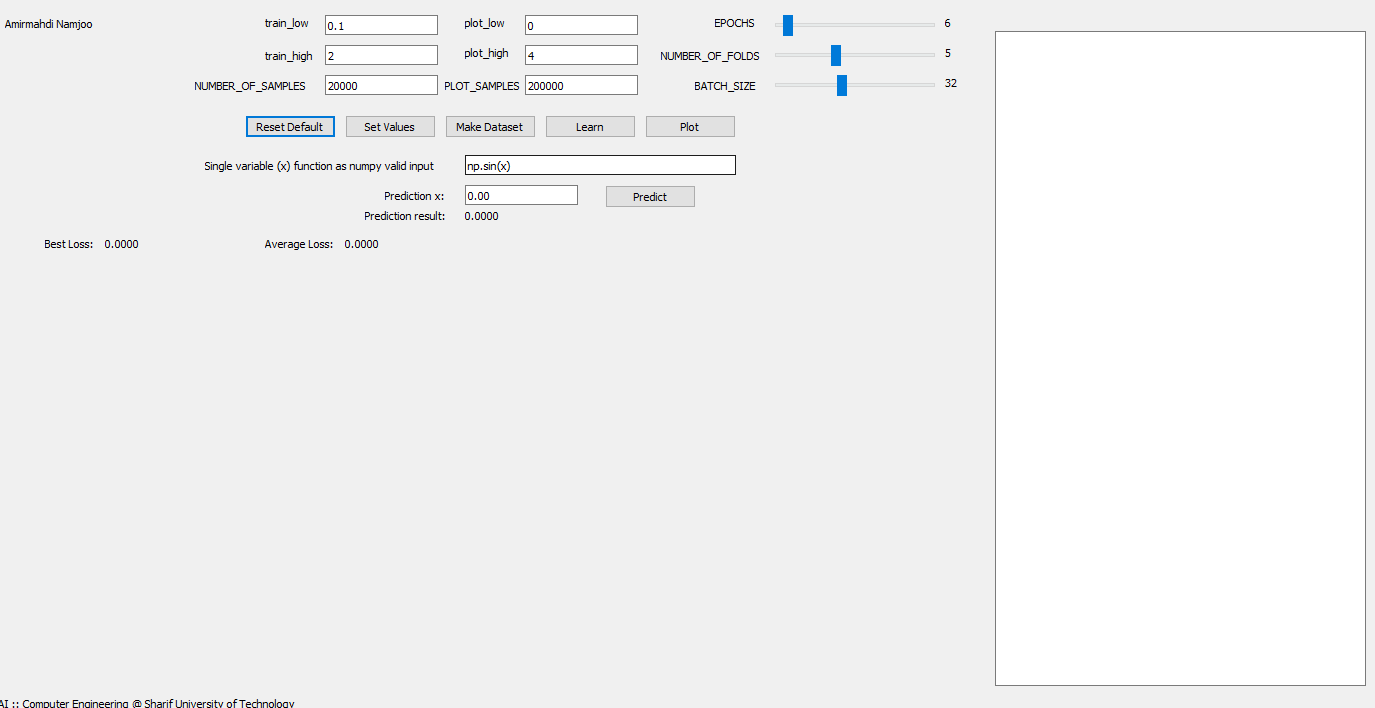
\includegraphics[width=1.1\textwidth]{pictures/24.png}

\end{center}

در این بخش می‌توان متغیرهای مختلف مسئله را تغییر داد. تابع ورودی باید به فرمی باشد که از نظر پایتون معتبر باشد. بهتر است توابع آن به صورت توابع numpy نوشته شوند و برای دسترسی به numpy هم از حرف مخفف np باید استفاده بشود.

برای اجرا، حتماً ابتدا روی \lr{Set Value }و سپس روی \lr{ Make Dataset} و در نهایت روی \lr{Learn} کلیک کنید.

با گزینه Plot امکان رسم نمودار وجود دارد و در نهایت با گزینه Predict هم می‌توان عدد مشخص شده را به عنوان $x$ به شبکه ورودی داده و مقدار خروجی شبکه را مشاهده کرد.


\newpage


\subsection{بخش دوم}

\begin{center}

 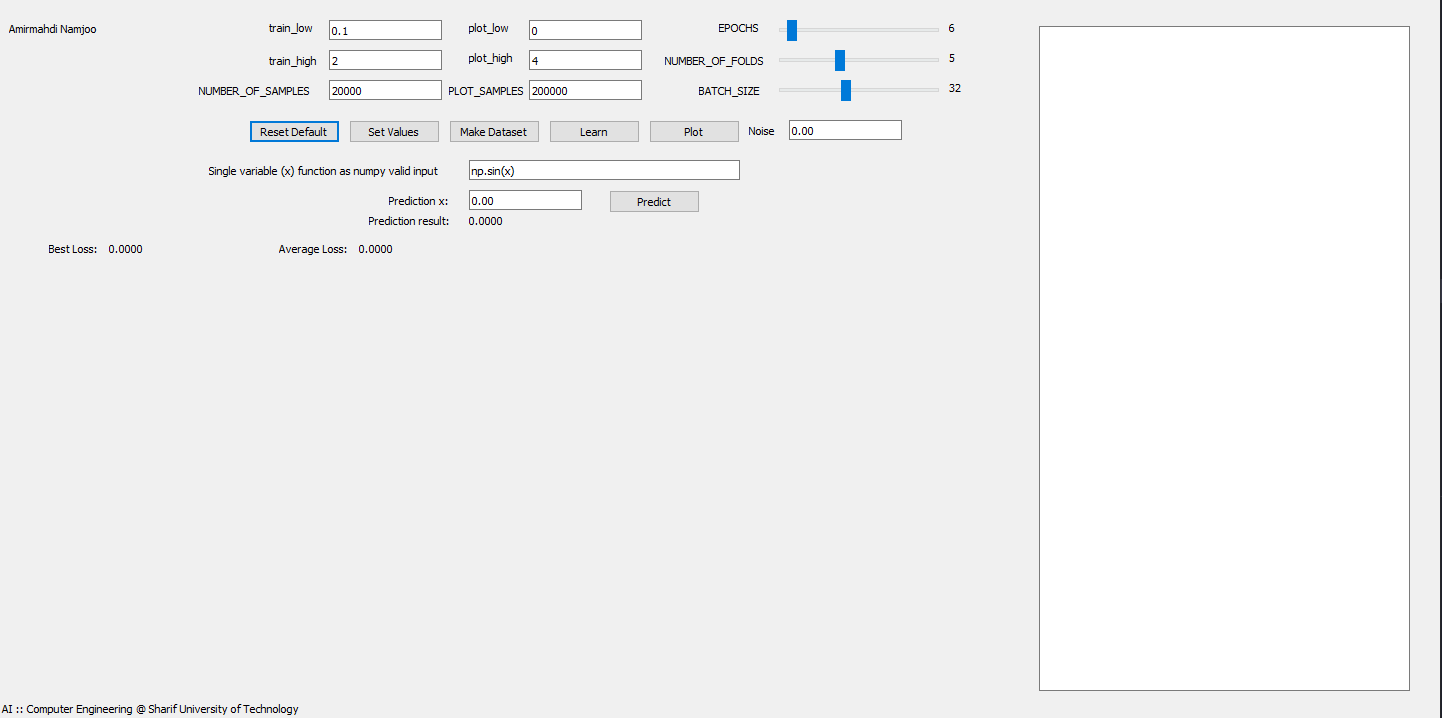
\includegraphics[width=1.1\textwidth]{pictures/25.png}

\end{center}

این بخش مشابه قسمت اول است فقط یک فیلد برای تعیین ضریب نویز هم اضافه شده است.



\newpage


\subsection{بخش سوم}

\begin{center}

 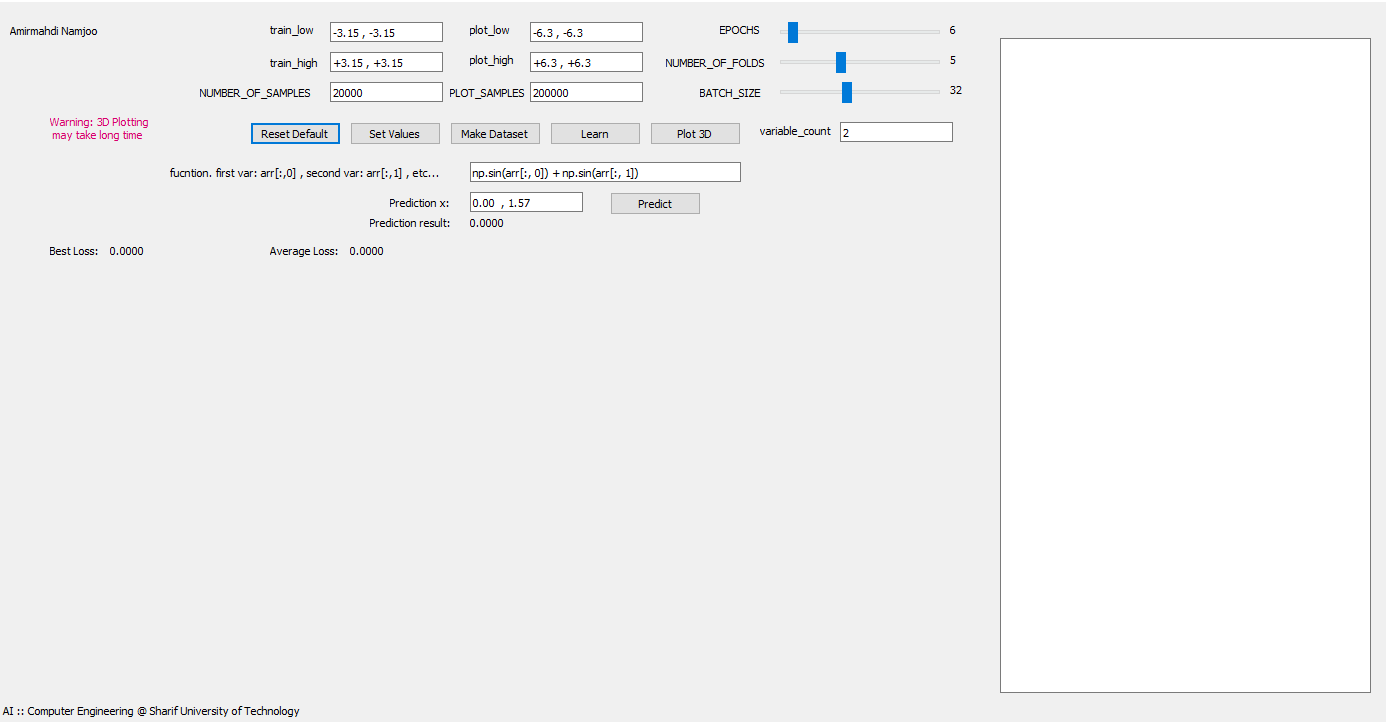
\includegraphics[width=1.1\textwidth]{pictures/26.png}

\end{center}

در این بخش امکان تعیین تعداد ورودی‌ها وجود دارد. تعداد ورودی‌ها باید حداقل 2 باشد.

در بخش‌هایی نظیر \lr{train\_low} باید به تعداد ورودی‌ها عددهایی که بازه‌های پایین و بالای مورد نیاز برای آموزش و رسم را مشخص می‌کنند، به صورت جدا شده با ویرگول وجود داشته باشند.

نکته مهم در مورد تابع این است که اسم متغیر را باید به شکل 
\begin{latin}
\begin{verbatim}
arr[:,1]
\end{verbatim}
\end{latin}

نمایش بدهید.

مثلا برای نمایش 
$sin(x) + sin(y) + sin(z)$ باید نوشت:

\begin{latin}
\begin{verbatim}
np.sin(arr[:,0]) + np.sin(arr[:,1]) * np.sin(arr[:,2])
\end{verbatim}
\end{latin}


برای قسمت پیش بینی مقادیر هم باید به تعداد ورودی‌های مورد نیاز، عددهای جدا شده با ویرگول قرار بگیرد.



\newpage



\subsection{بخش چهارم}

\begin{center}

 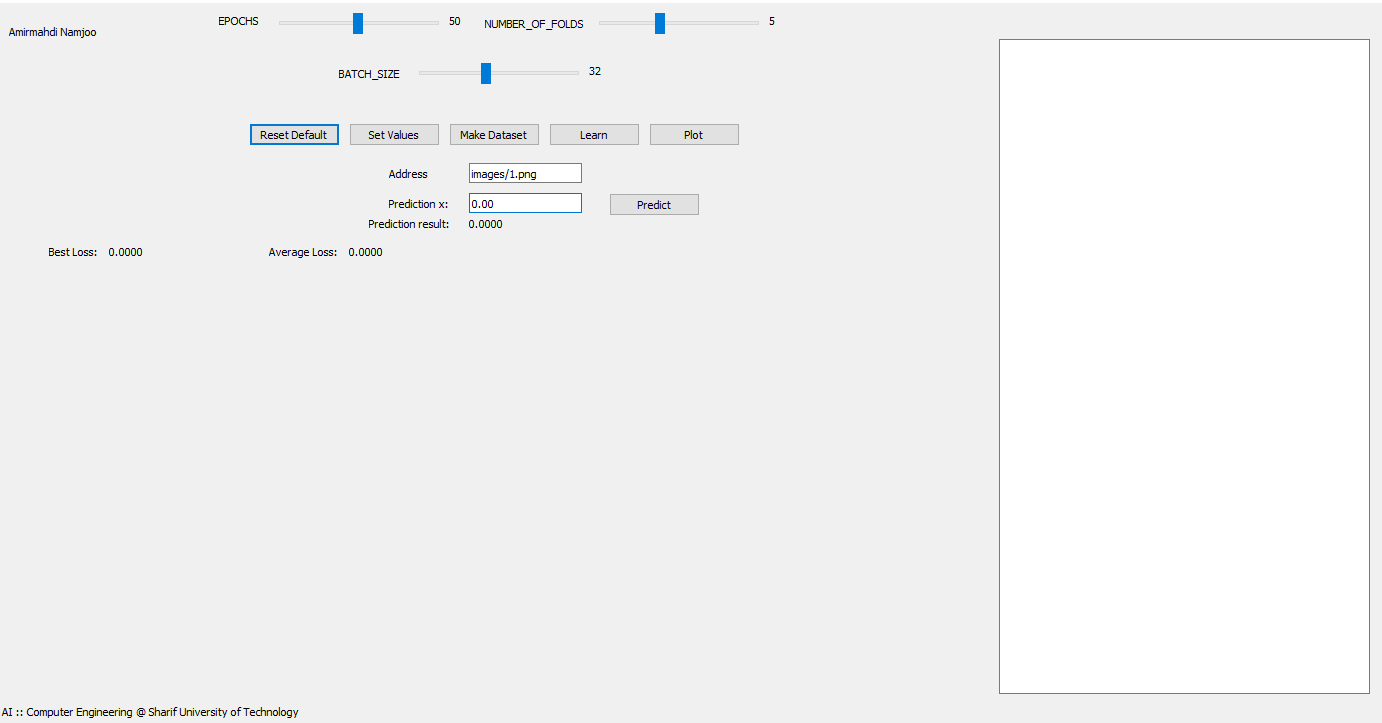
\includegraphics[width=1.1\textwidth]{pictures/27.png}

\end{center}

تنها نکته قابل توجه و متفاوت در این قسمت فیلد آدرس است که در آن باید آدرس relative عکسی که باید لود شود را نسبت به فایل \lr{Regressor.py} مشخص کرد.


\subsection{بخش پنجم}

\begin{center}

 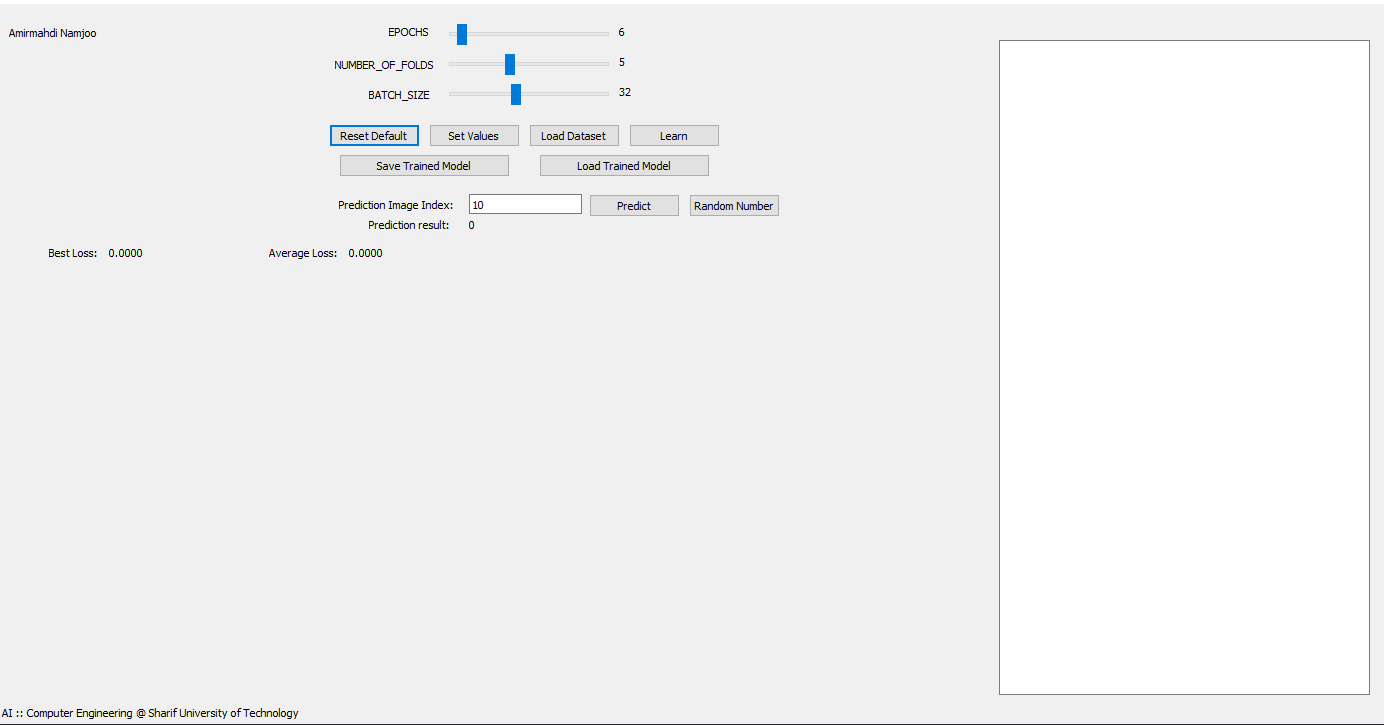
\includegraphics[width=1.1\textwidth]{pictures/28.png}

\end{center}
نکته قابل توجه در این بخش این است که می‌توانید با وارد کردن اندیس یک عکس بعد از آموزش شبکه (یا لود شدن شبکه از پیش آموزش داده شده) نتیجه پیش بینی شبکه و خود عکس را مشاهده کرد. می‌توانید با کلیک روی گزینه \lr{Random Number} هم یک اندیس تصادفی ایجاد کنید.


گزینه‌هایی هم قرار داده شده که می‌توانند مدل آموزش دیده شده را روی کامپیوتر ذخیره کرده و مدل از پیش ذخیره شده را لود کنند تا نیاز به آموزش مجدد نباشد.


 

\newpage


\subsection{بخش ششم}

\begin{center}

 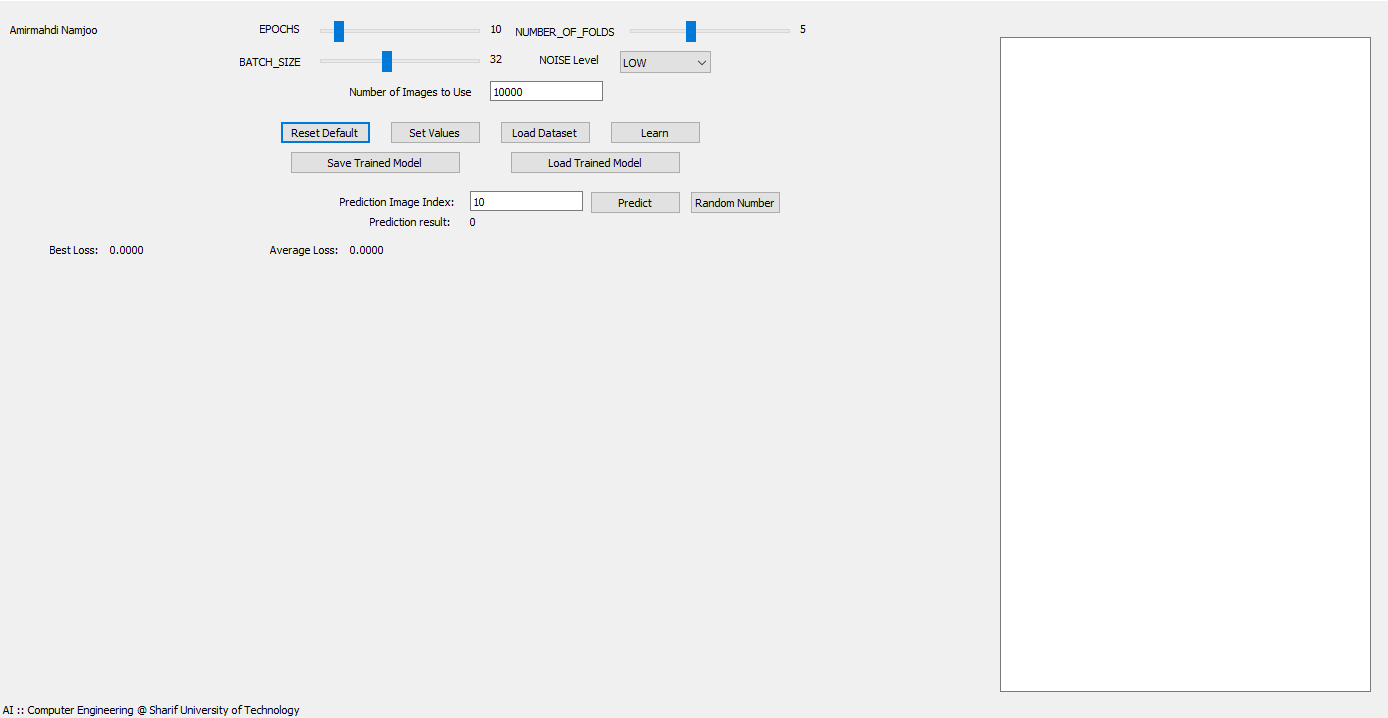
\includegraphics[width=1.1\textwidth]{pictures/29.png}

\end{center}

در این بخش علاوه بر موارد مرسوم قبلی، امکان انتخاب سطح نویز عکس و همچنین تعداد عکس‌هایی که برای کل فرآیند استفاده خواهند شد نیز وجود دارد.

بعد از طی فرآیند آموزش هم برای مشاهده عکس‌ها در فیلد قرار داده شده، می‌توانید چند عدد که با ویرگول جدا شده‌اند را وارد کنید تا در نمودار نهایی، شاهد نتیجه اجرای شبکه عصبی بر روی چندین عکس مختلف باشید.






\newpage



\section{چالش‌ها}

در این پروژه با چالش‌های مختلفی رو به رو شدم.

بخش اول چالش مربوط به راه اندازی و یادگیری Keras بود. از طریق مشاهده چندین ویدیو در اینترنت و همچنین مطالعه سایت \lr{keras.io} تا حد خوبی با آن آشنا شدم. یک چالش در این بخش کار نصب کردن tensorflow بود. نصب خود آن دردسر زیادی نداشت ولی از آن جایی که لپ تاپ من از کارت گرافیک \lr{GTX1070} بهره می‌برد، علاقه داشتم که حالت GPU آن را هم تست کنم و زمانی را صرف دانلود چندین فایل مختلف از سایت Nvidia کردم تا در نهایت امکان اجرای آن روی GPU هم برای من مهیا شد. هر چند اکثر بخش‌های این پروژه به دلیل این که ساختار کلی شبکه نسبتاً ساده است، عملکرد GPU و CPU تفاوت خیلی معناداری نمی‌کرد. مخصوصاً این که به هر حال ارتباط بین GPU و CPU مقداری سربار عملکردی ایجاد می‌کند و استفاده از GPU وقتی به صرفه است که ساختار شبکه آن‌قدر پیچیده باشد که اثر موازی سازی کارها در GPU بر سربار عملکردی ارتباط بین CPU و GPU غلبه کند.

یکی دیگر از چالش‌ها این بود که در مورد انواع توابع فعال ساز مقداری مطالعه کنم تا در نهایت برای هر بخش پروژه از توابع فعال ساز دیگر استفاده کنم.

علاوه بر این‌ها، یک چالش عمده دیگر که با آن رو به رو شدم، ساخت GUI بود. از آن جایی که تا به حال با پایتون GUI نساخته بودم، با جست و جو در اینترنت به فریمورک PyQt رسیدم که بر اساس فریمورک Qt زبان C++ ساخته شده است و نرم‌افزارهایی نظیر \lr{Qt Creator} و \lr{Qt Designer} برای آن وجود دارند که به کمک آن‌ها می‌توان ظاهر کلی را به صورت گرافیکی طراحی کرده و سپس از طریق کد پایتون، عملکردهایی که هر دکمه و اجزای رابط کاربری باید داشته باشند را به آن‌ها Bind کرد. با مطالعه چندین منبع، در نهایت موفق به ساخت رابط کاربری گرافیکی نسبتاً خوب هم برای پروژه خود شدم.





\end{document}














